\documentclass[../main.tex]{subfiles}

\begin{document}
\section{Results}\label{sec:results}

Here we present figures showing the results of the simulations we have produced of the solar system. 

\subsection{Earth-Sun}

We simulate the Earth-Sun system with gravity acting on both the Sun and the Earth, comparing the velocity Verlet method with the forward Euler method. This is shown in \cref{fig:earth-sun-verlet-vs-euler}. The Euler-Cromer method was also used for comparison, shown in \cref{eq:euler-cromer}.

\iffalse
\begin{figure}[htb!]
    \centering
    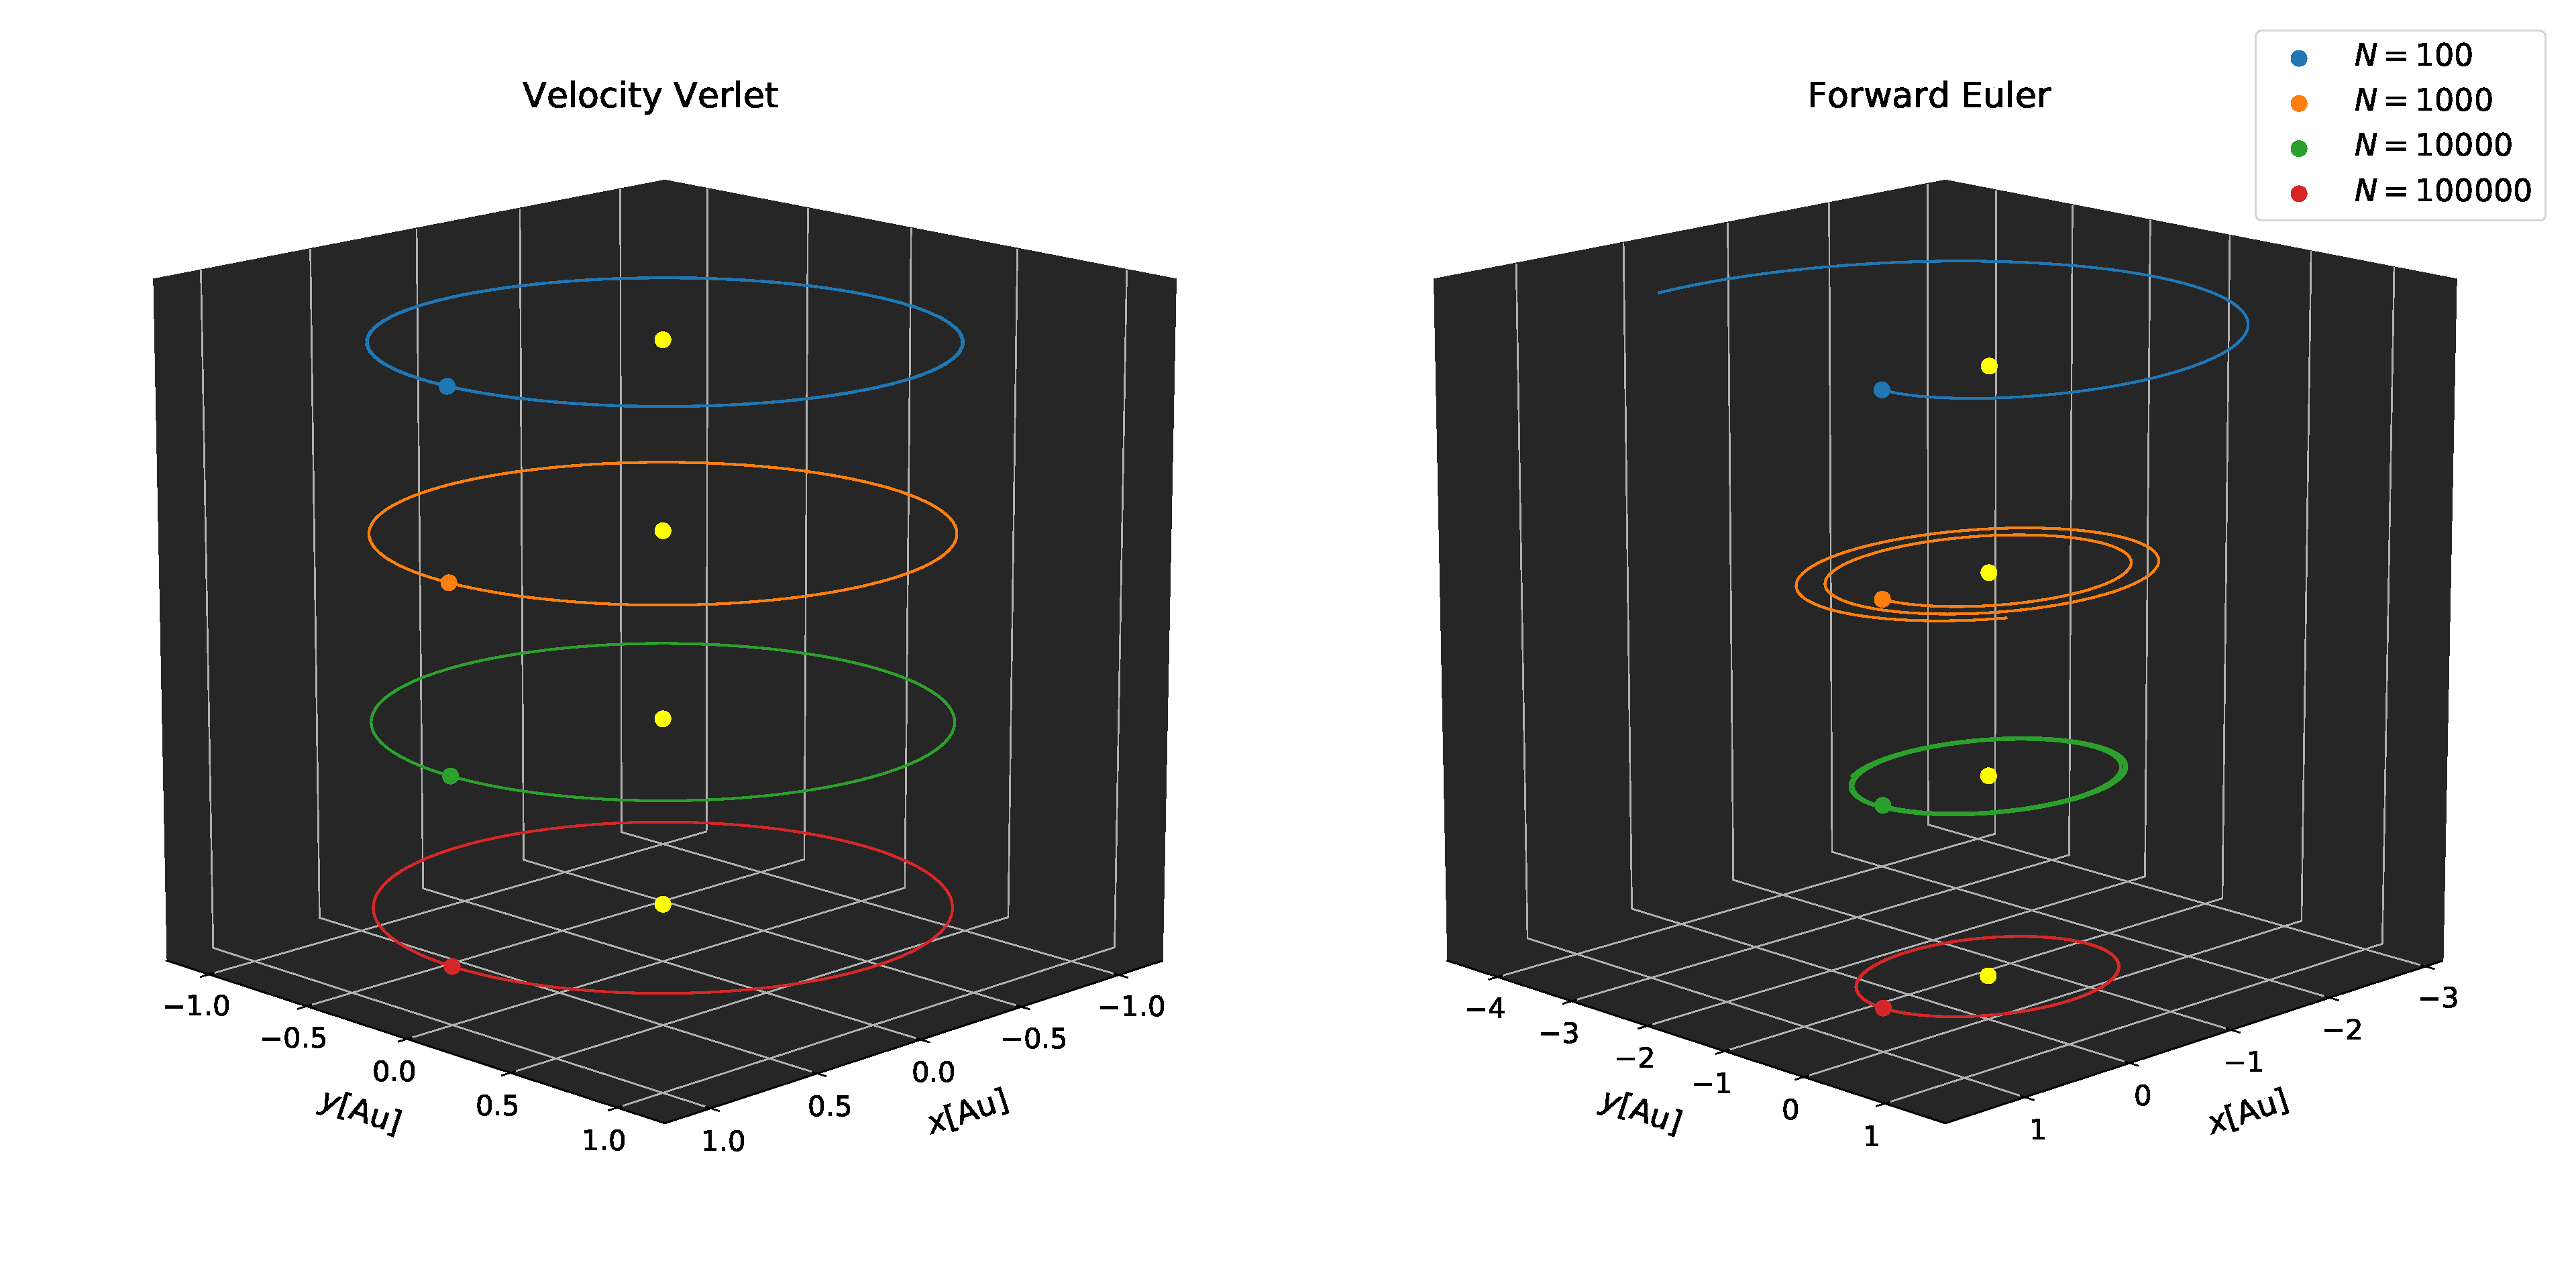
\includegraphics[trim=2cm 0.cm 0.cm 0.cm, clip,width=\textwidth]{../figures/stability.pdf}
    \caption{Here is the Earth-Sun system simulated over 3 years using the Euler and Verlet methods. The Earth does not form a closed orbit for the Forward Euler method, and is slowly escaping the gravitational well of the Sun, especially for small numbers simulation points. The velocity Verlet method remains stable at even very few points.}
    \label{fig:earth-sun-verlet-vs-euler}
\end{figure}

\begin{figure}[htb!]
    \centering
    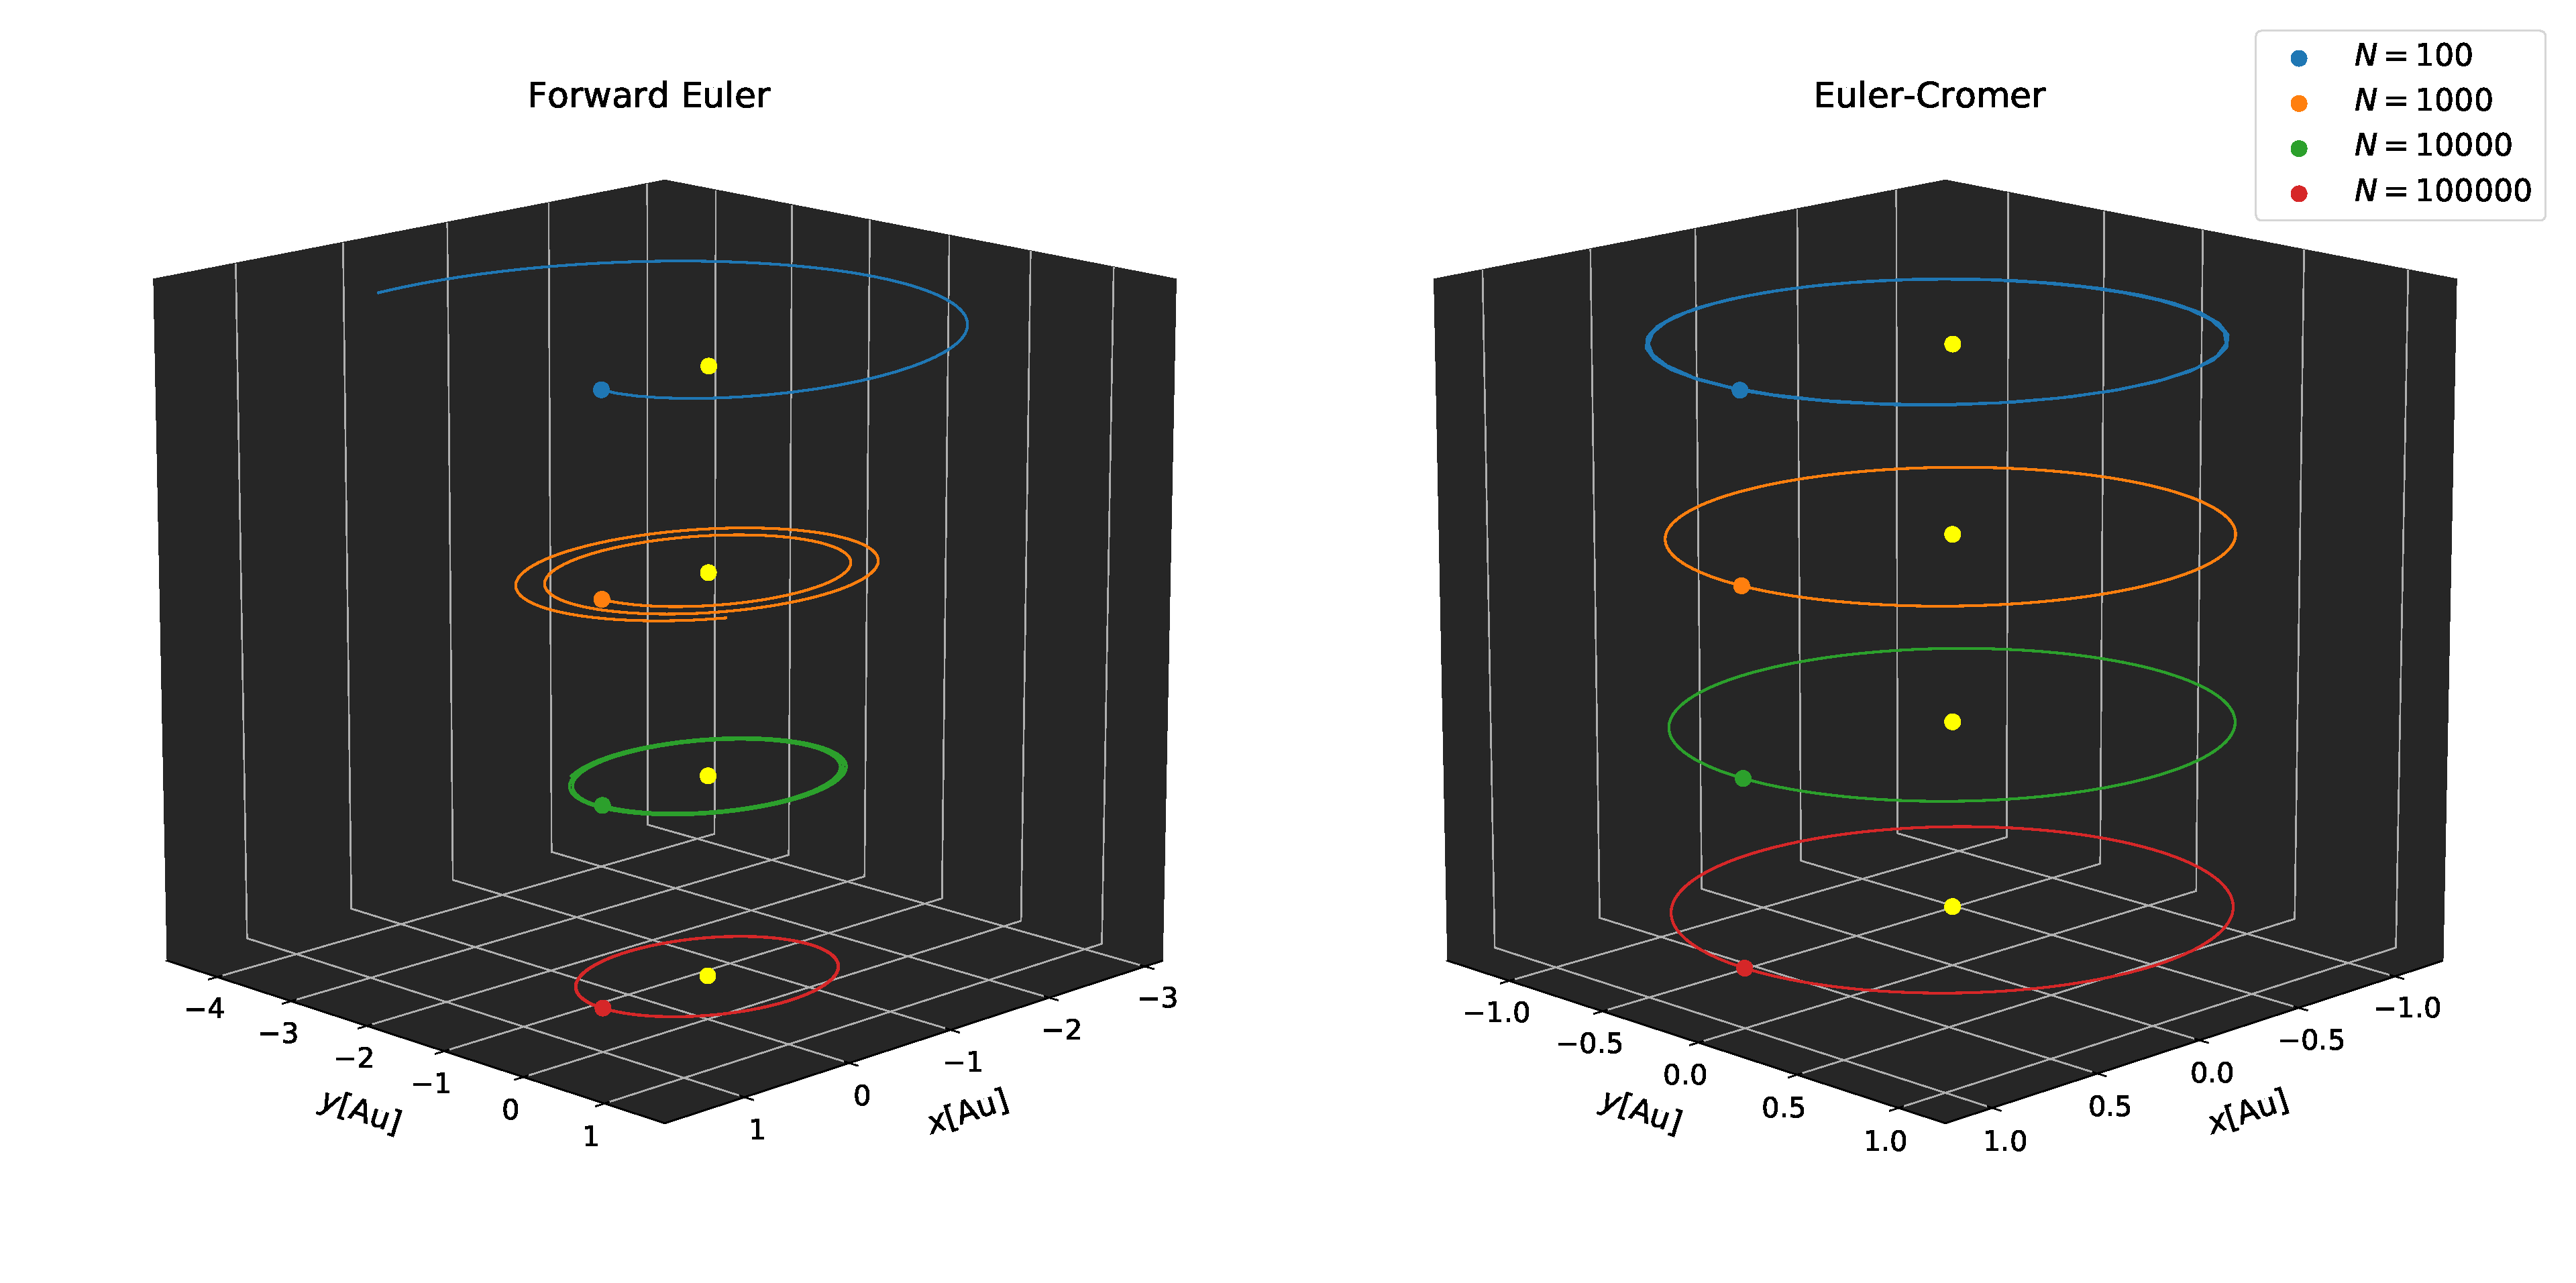
\includegraphics[trim=30cm 0.cm 0.cm 0.cm, clip,width=0.6\textwidth]{../figures/euler_vs_cromer.pdf}
    \caption{This figure shows the same simulation as \cref{fig:earth-sun-verlet-vs-euler}, but with the Euler-Cromer method. The Euler-Cromer method is stable even for small numbers of time steps as expected for a symplectic method.}
    \label{fig:earth-sun-cromer-vs-euler}
\end{figure}
\fi

\begin{figure}[htb!]
    \centering
    \begin{subfigure}[b]{\textwidth}
    \centering
    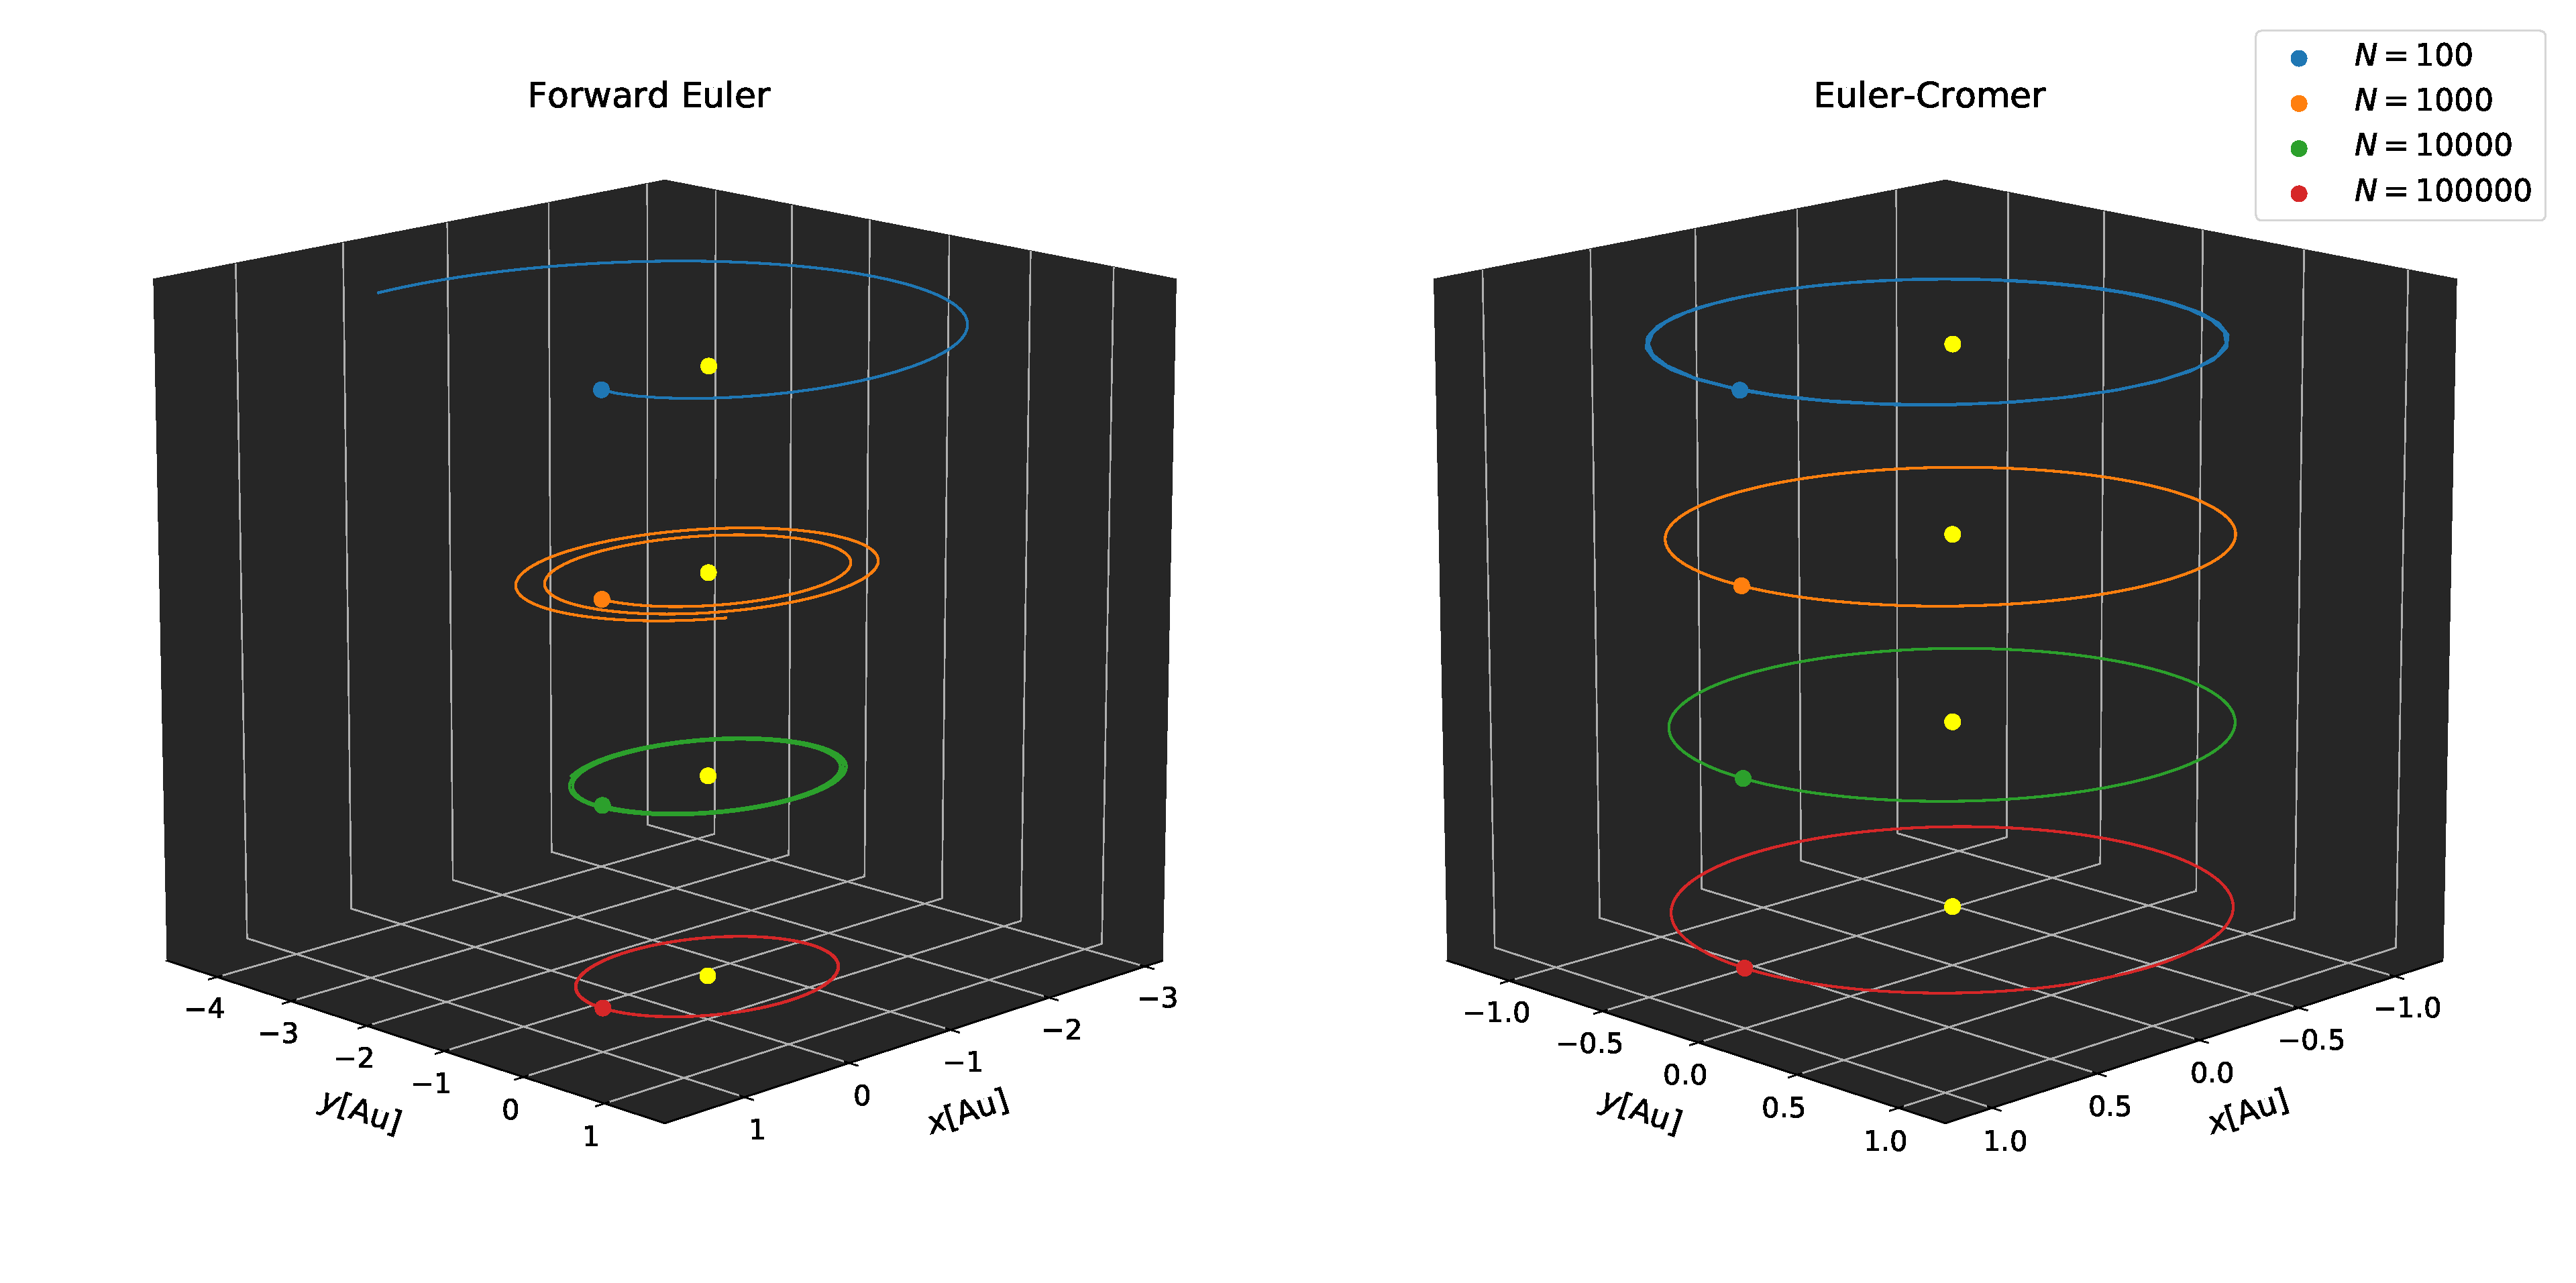
\includegraphics[trim=30cm 0.cm 0.cm 0.cm, clip,width=0.6\textwidth]{../figures/euler_vs_cromer.pdf}
    \caption{}
    \label{fig:earth-sun-cromer-vs-euler}
    \end{subfigure}
    
    \begin{subfigure}[b]{\textwidth}
    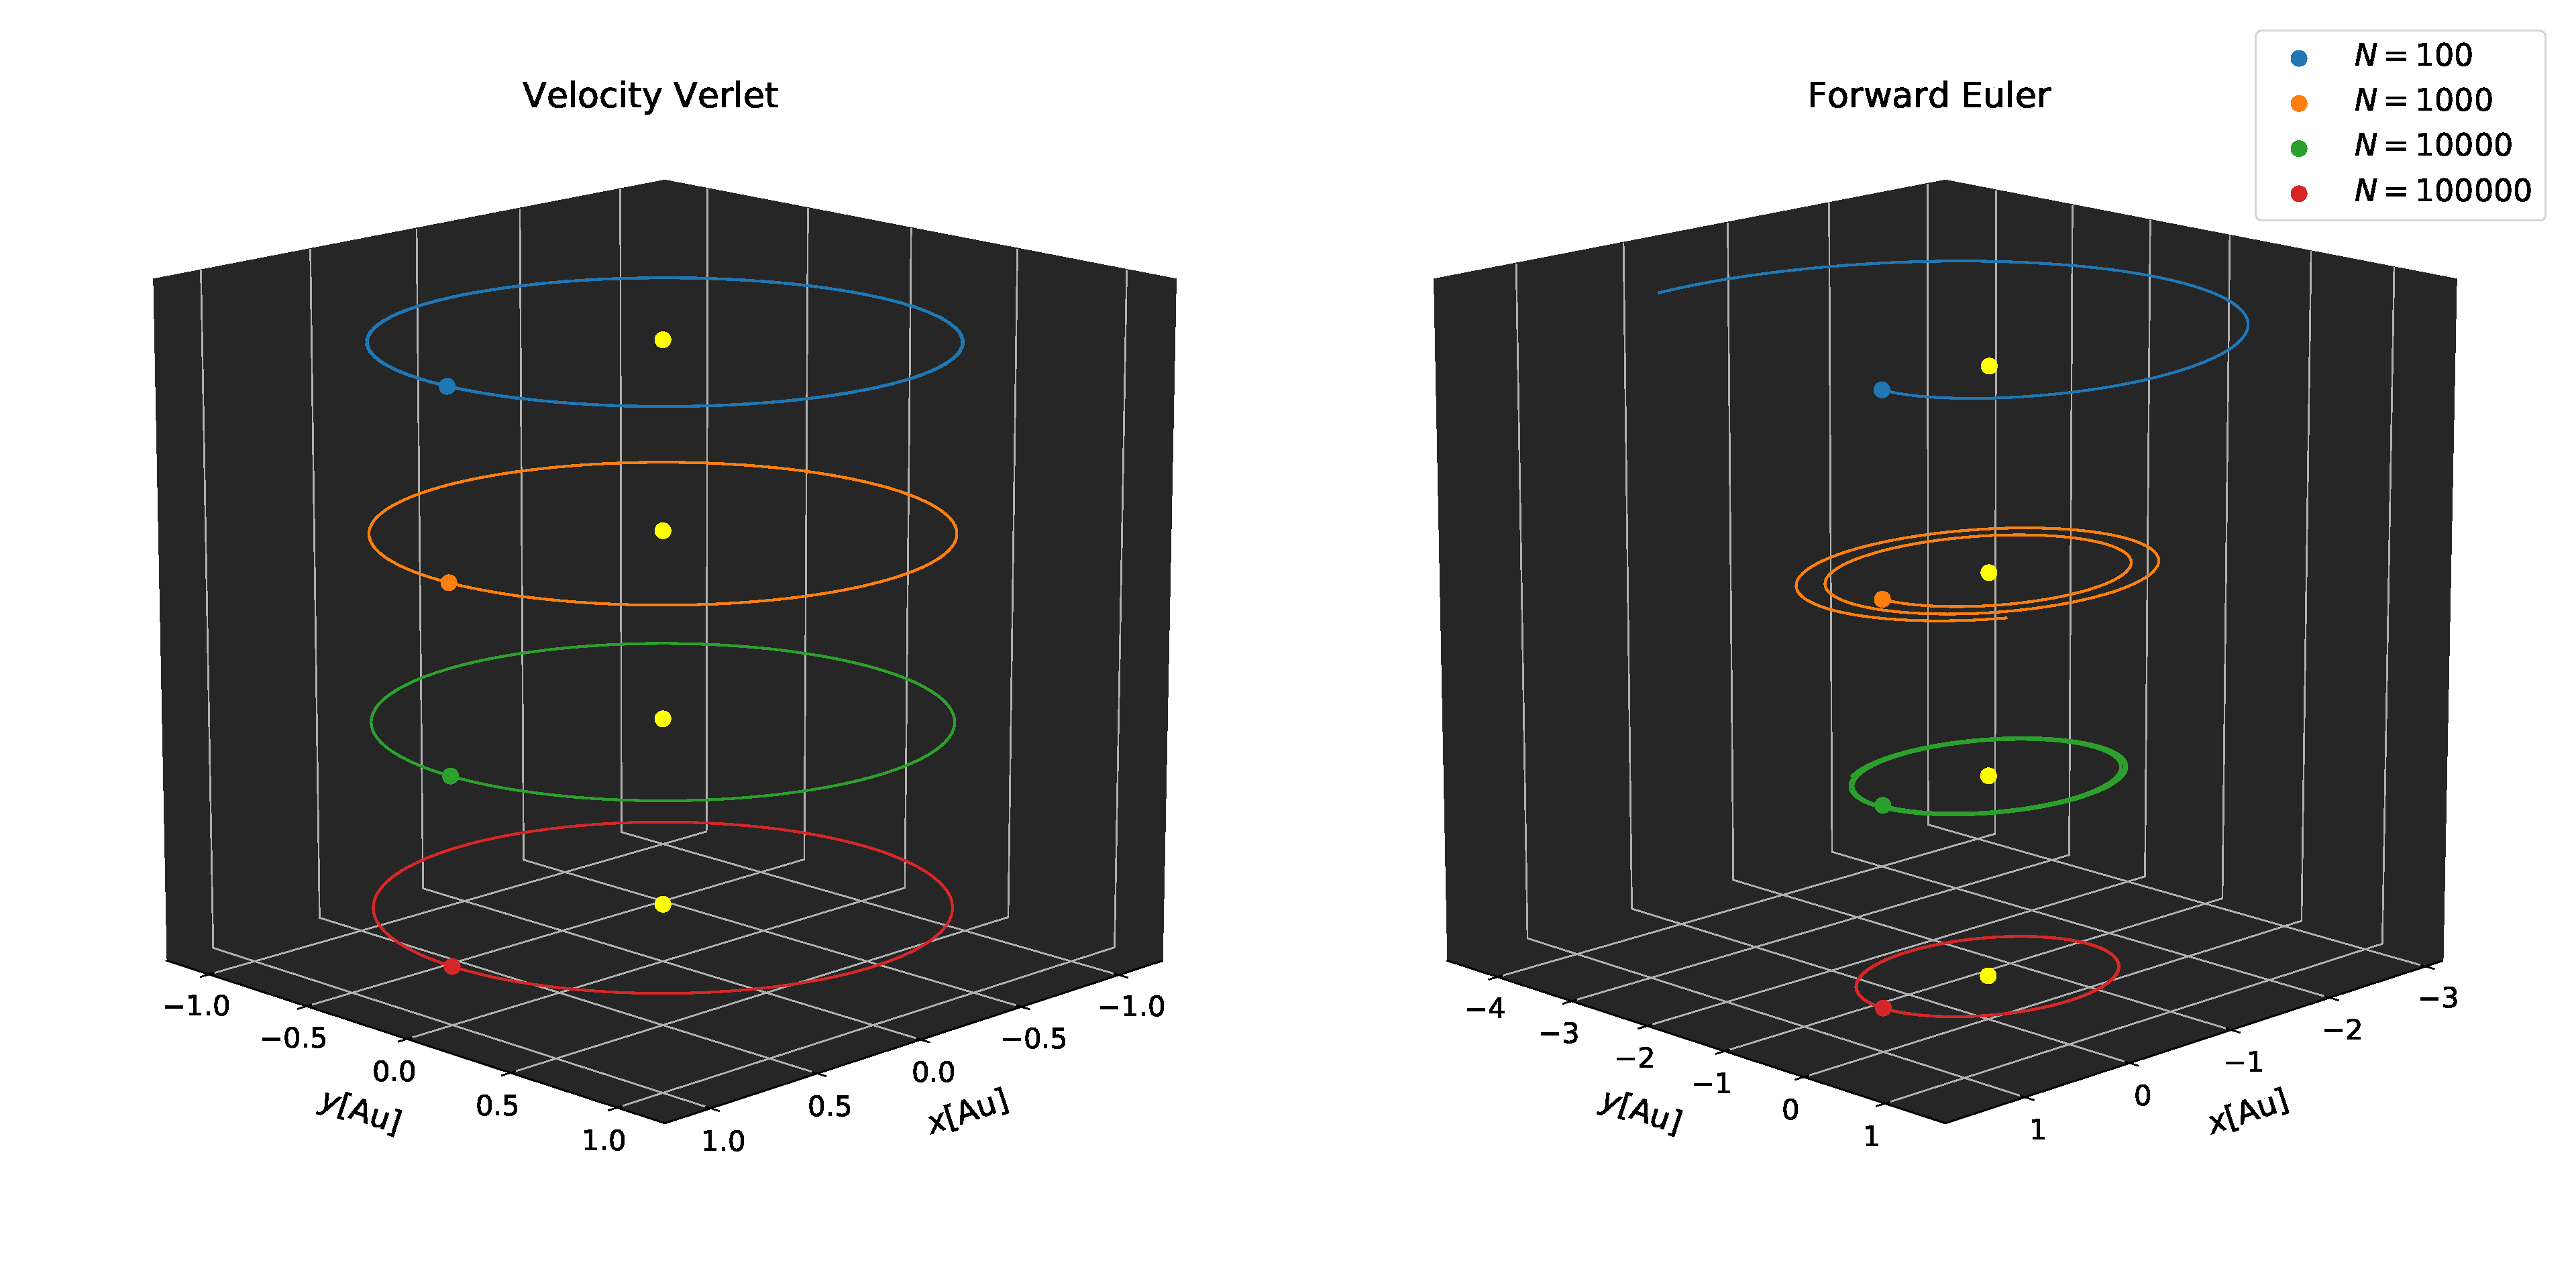
\includegraphics[trim=2cm 0.cm 0.cm 0.cm, clip,width=\textwidth]{../figures/stability.pdf}
    \caption{}
    \label{fig:earth-sun-verlet-vs-euler}
    \end{subfigure}
    \caption{(a) This figure shows the same simulation as \cref{fig:earth-sun-verlet-vs-euler}, but with the Euler-Cromer method. The Euler-Cromer method is stable even for small numbers of time steps as expected for a symplectic method. (b) Here is the Earth-Sun system simulated over 3 years using the Euler and Verlet methods. The Earth does not form a closed orbit for the Forward Euler method, and is slowly escaping the gravitational well of the Sun, especially for small numbers simulation points. The velocity Verlet method remains stable at even very few points. }
    
\end{figure}



For circular motion we expect from \cref{eq:GM-sun} and \cref{eq:circular-velocity} that the velocity that yields circular motion for the Earth around the Sun is $2 \pi \frac{\text{AU}}{\text{Year}}$. This is also the velocity used in the various simulations with circular motion of the Earth.

\subsection{Algorithm Timing}

Running 10 simulations of three years of the Earth-Sun system yields average timings of $\approx 22.54$ seconds for the velocity Verlet method, and $\approx 20.33$ seconds for the forward Euler method. The difference is surprisingly small, despite the Verlet method requiring ostensibly more than twice as many floating point operations as the Euler method. Since the velocity Verlet method is also much more accurate with a total error $\mathcal{O}(h^2)$ compared with the Euler method at $\mathcal{O}(h)$, we use the velocity Verlet method in all subsequent simulations of the solar system.

\subsection{Generalized Newtonian Gravity}

Generalizing the gravitational force as in \cref{eq:gravity-generalized}, we simulated the Earth-Sun system over three years for varying values of $\beta$ as plotted in \cref{fig:varying-beta}.

\begin{figure}[htb!]
    \centering
    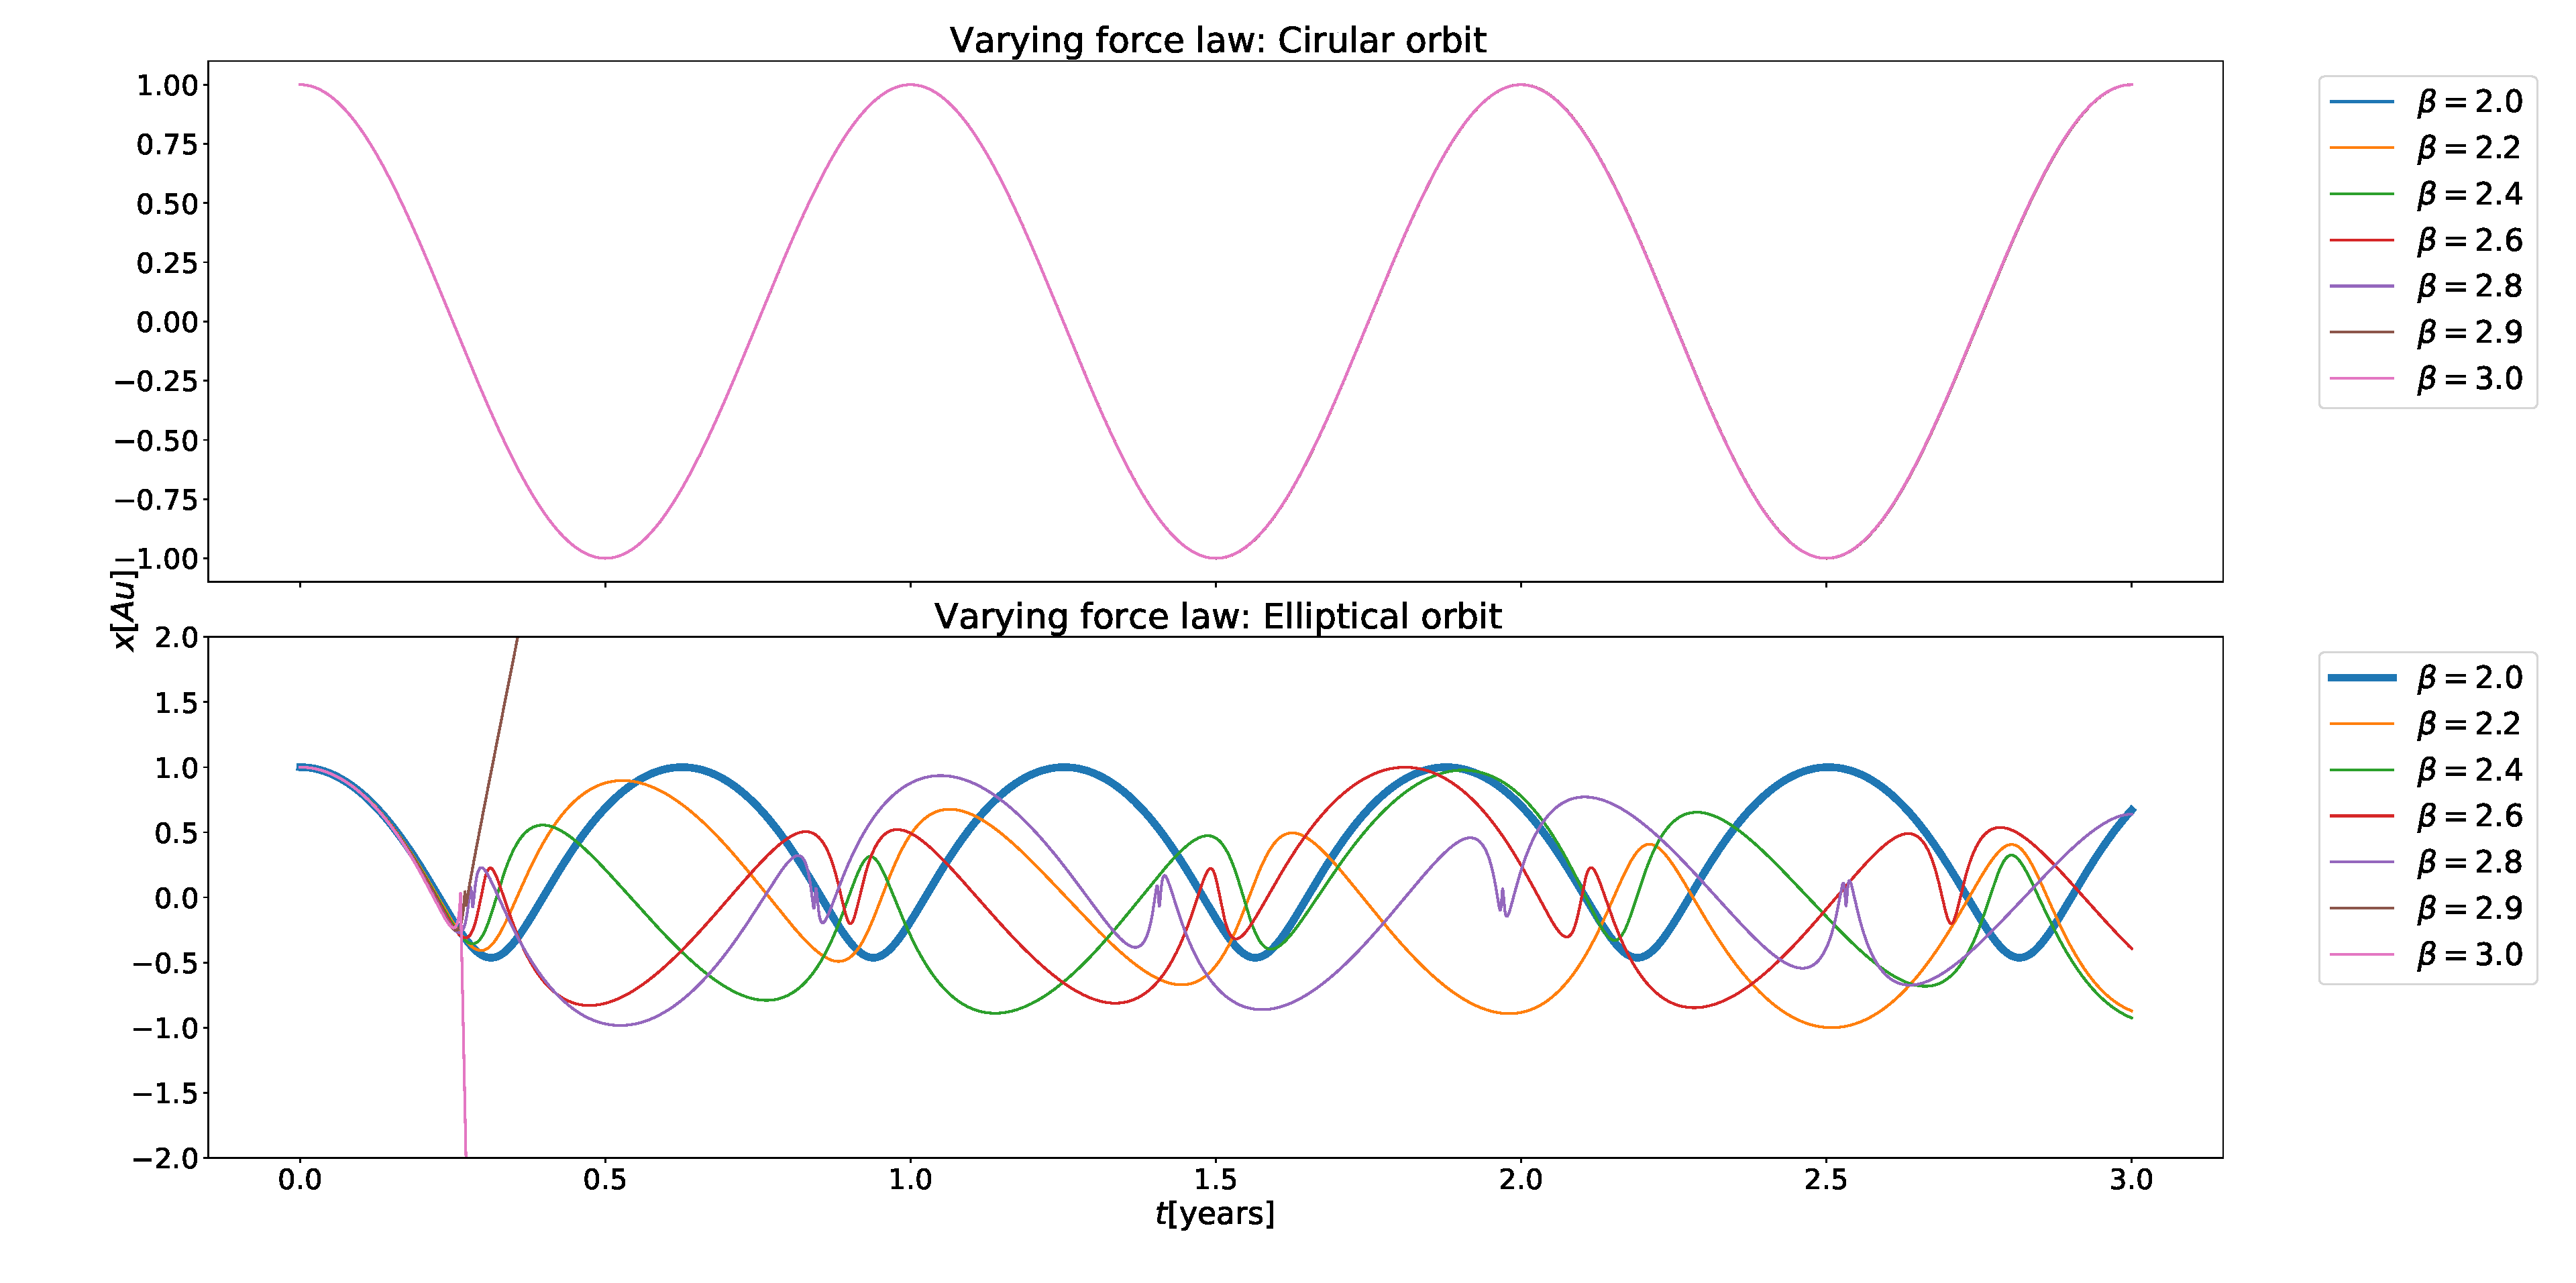
\includegraphics[trim=0cm 0.cm 0.cm 0.cm, clip,width=\textwidth]{../figures/varying_force.pdf}
    \caption{This plot shows the $x$-axis movement of the Earth in the Sun-Earth system simulated over three years, with varying values of $\beta$ for generalized Newtonian gravity. For an elliptical orbit, the system varies greatly with $\beta$, and loses stability for $\beta \xrightarrow{} 3$.}
    \label{fig:varying-beta}
\end{figure}

\subsection{Escape Velocity}

To find the escape velocity of the Earth in the Earth-Sun system numerically, simple trial and error was used. The results are shown in \cref{fig:earth-escape-velocity}, and the final value of the initial velocity $v_0$ that was sufficient for the Earth to leave the solar system is $v_0 = 8.885764876 \frac{\text{AU}}{\text{year}}$. Comparing with the analytic value $2 \sqrt{2} \pi \approx 8.885765876 \frac{\text{AU}}{\text{year}}$, we see a very small difference of order $10^{-6}$.

\begin{figure}[htb!]
    \centering
    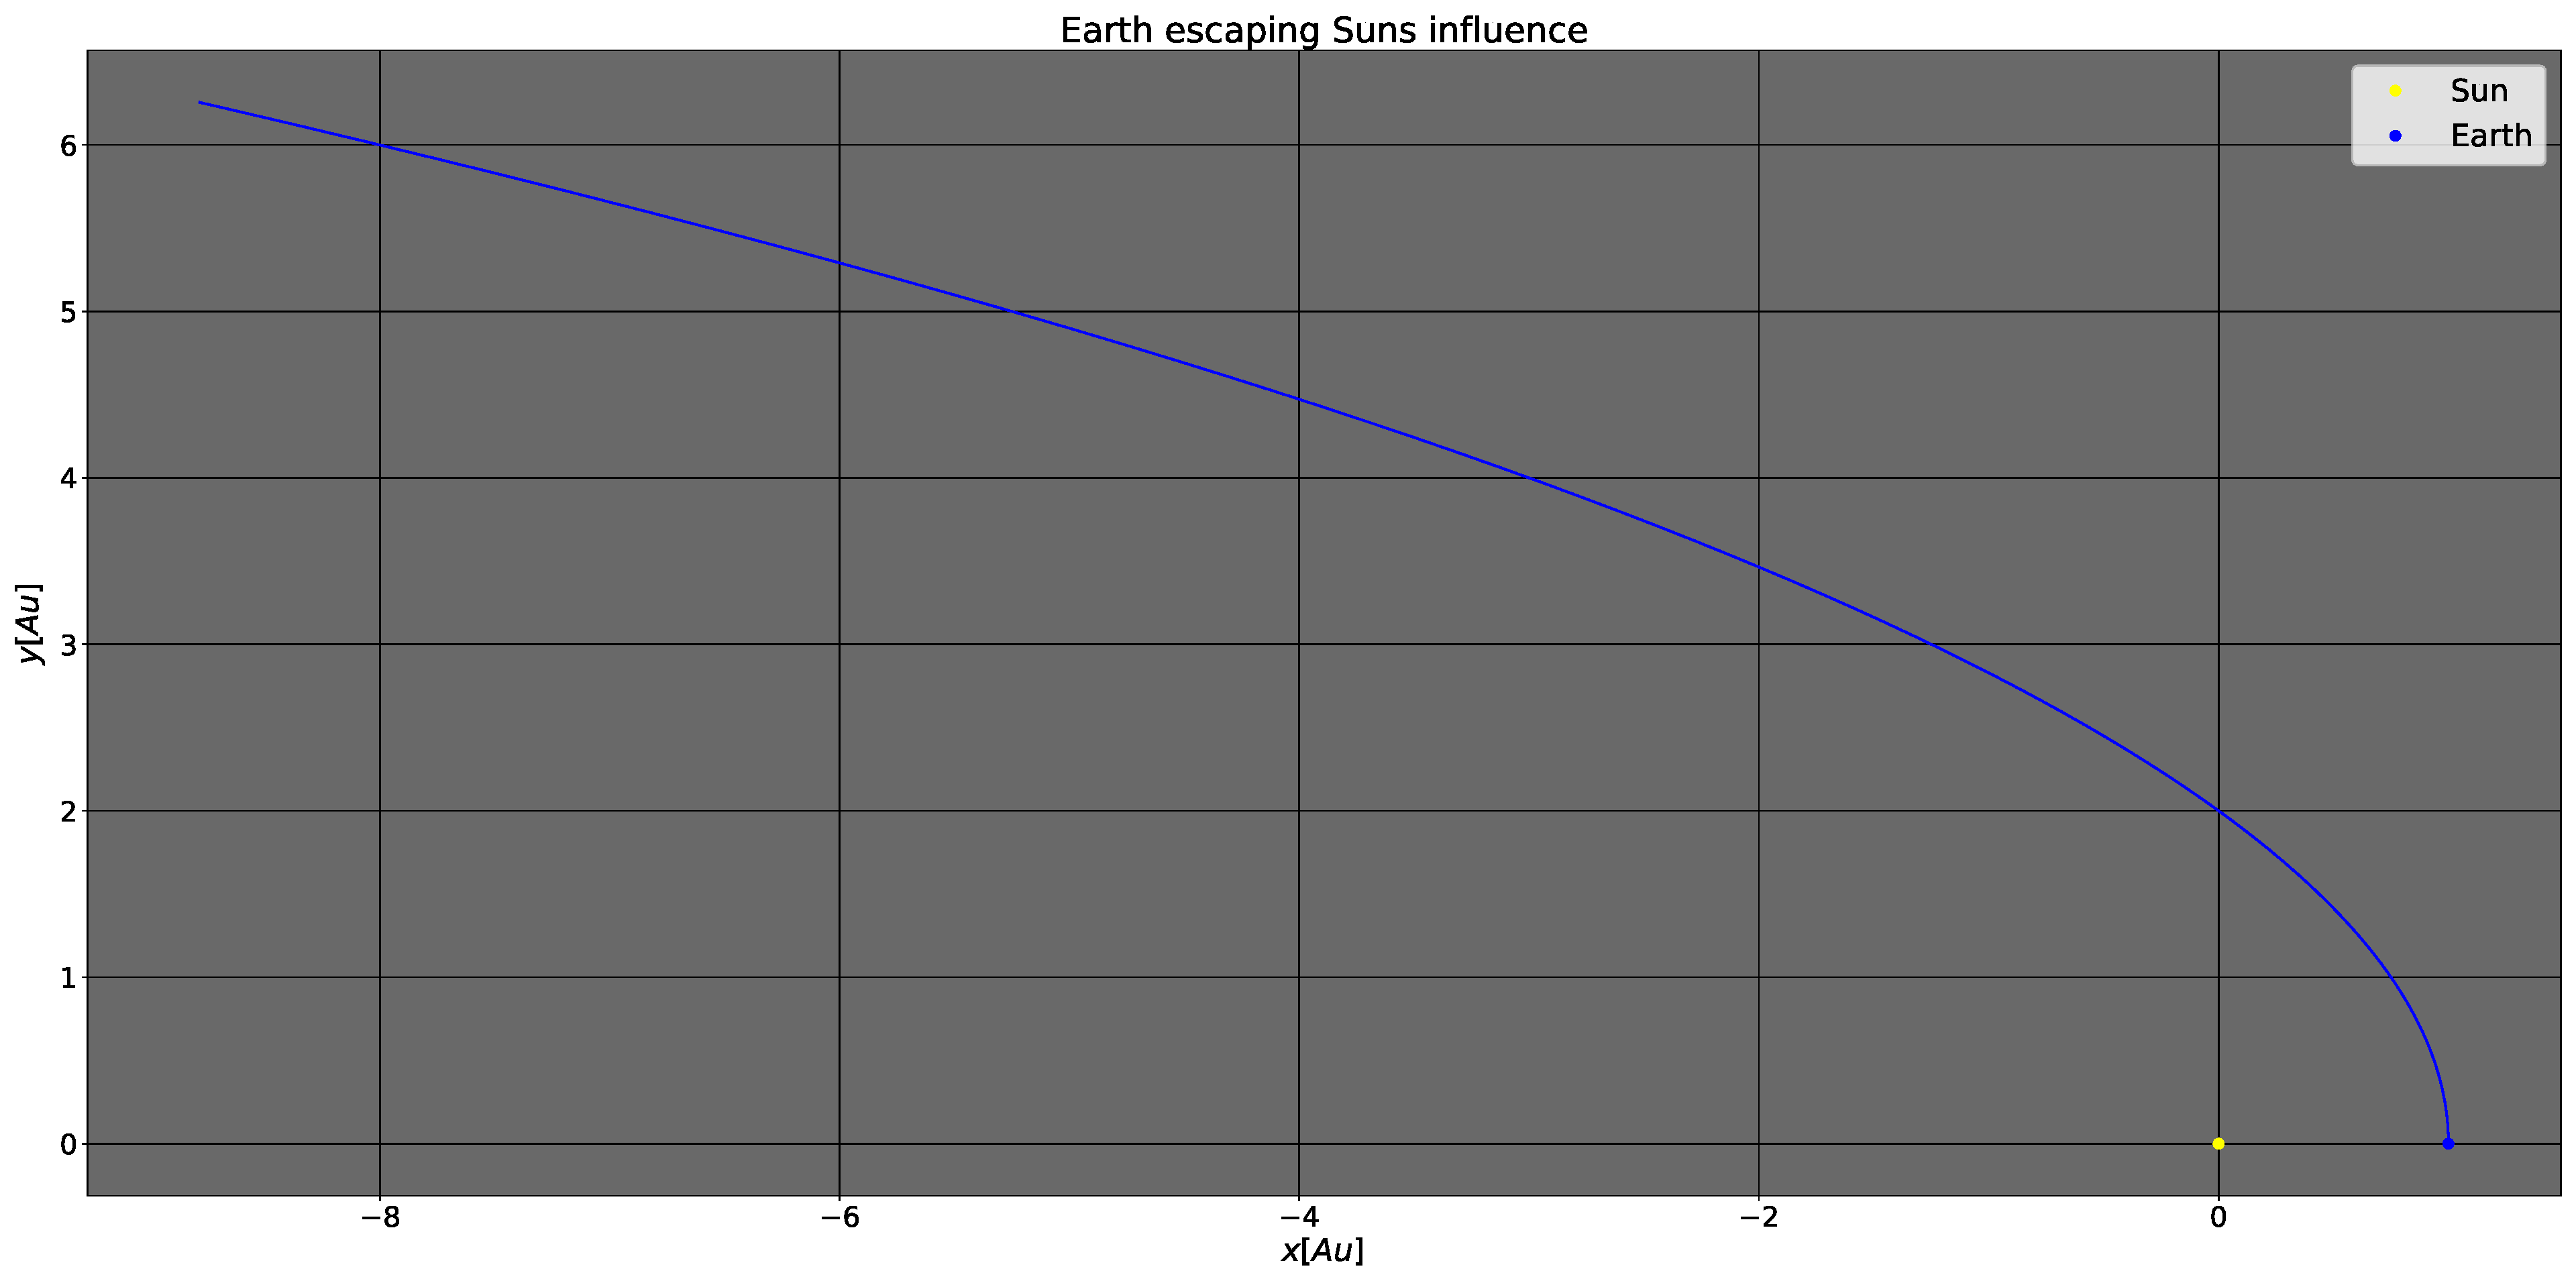
\includegraphics[trim=5.cm 0.cm 0.cm 0.cm, clip,width=0.8\textwidth]{../figures/escape.pdf}
    \caption{Pictured is a simulation over 3 years, with the initial velocity of the earth set to $v_0 = 8.885764876 \frac{\text{AU}}{\text{year}}$. By trial and error, this value seems to be enough for the Earth to leave the Solar system.}
    \label{fig:earth-escape-velocity}
\end{figure}

\subsection{Three-body Problem}
We have implemented a model consisting of the Sun, Earth and Jupiter, employing the velocity Verlet method. \Cref{fig:three-body-problem} shows the simulated orbits of the celestial bodies in our model for 10 years. The top subfigure shows the simulation with Jupiter's usual mass, $M_j$. We also model the scenarios where Jupiter's mass is $10M_j$ and $1000M_j$, which is shown in the middle and bottom subfigure, respectively. As one can see from \cref{fig:three-body-problem}, a mass of $10M_j$ would drag the Earth closer to the Sun, while a mass of $1000M_j$ causes the Earth to leave the system entirely, while Jupiter and the Sun start orbiting each other, similar to a binary star system. 

\begin{figure}[htb!]
    \centering
    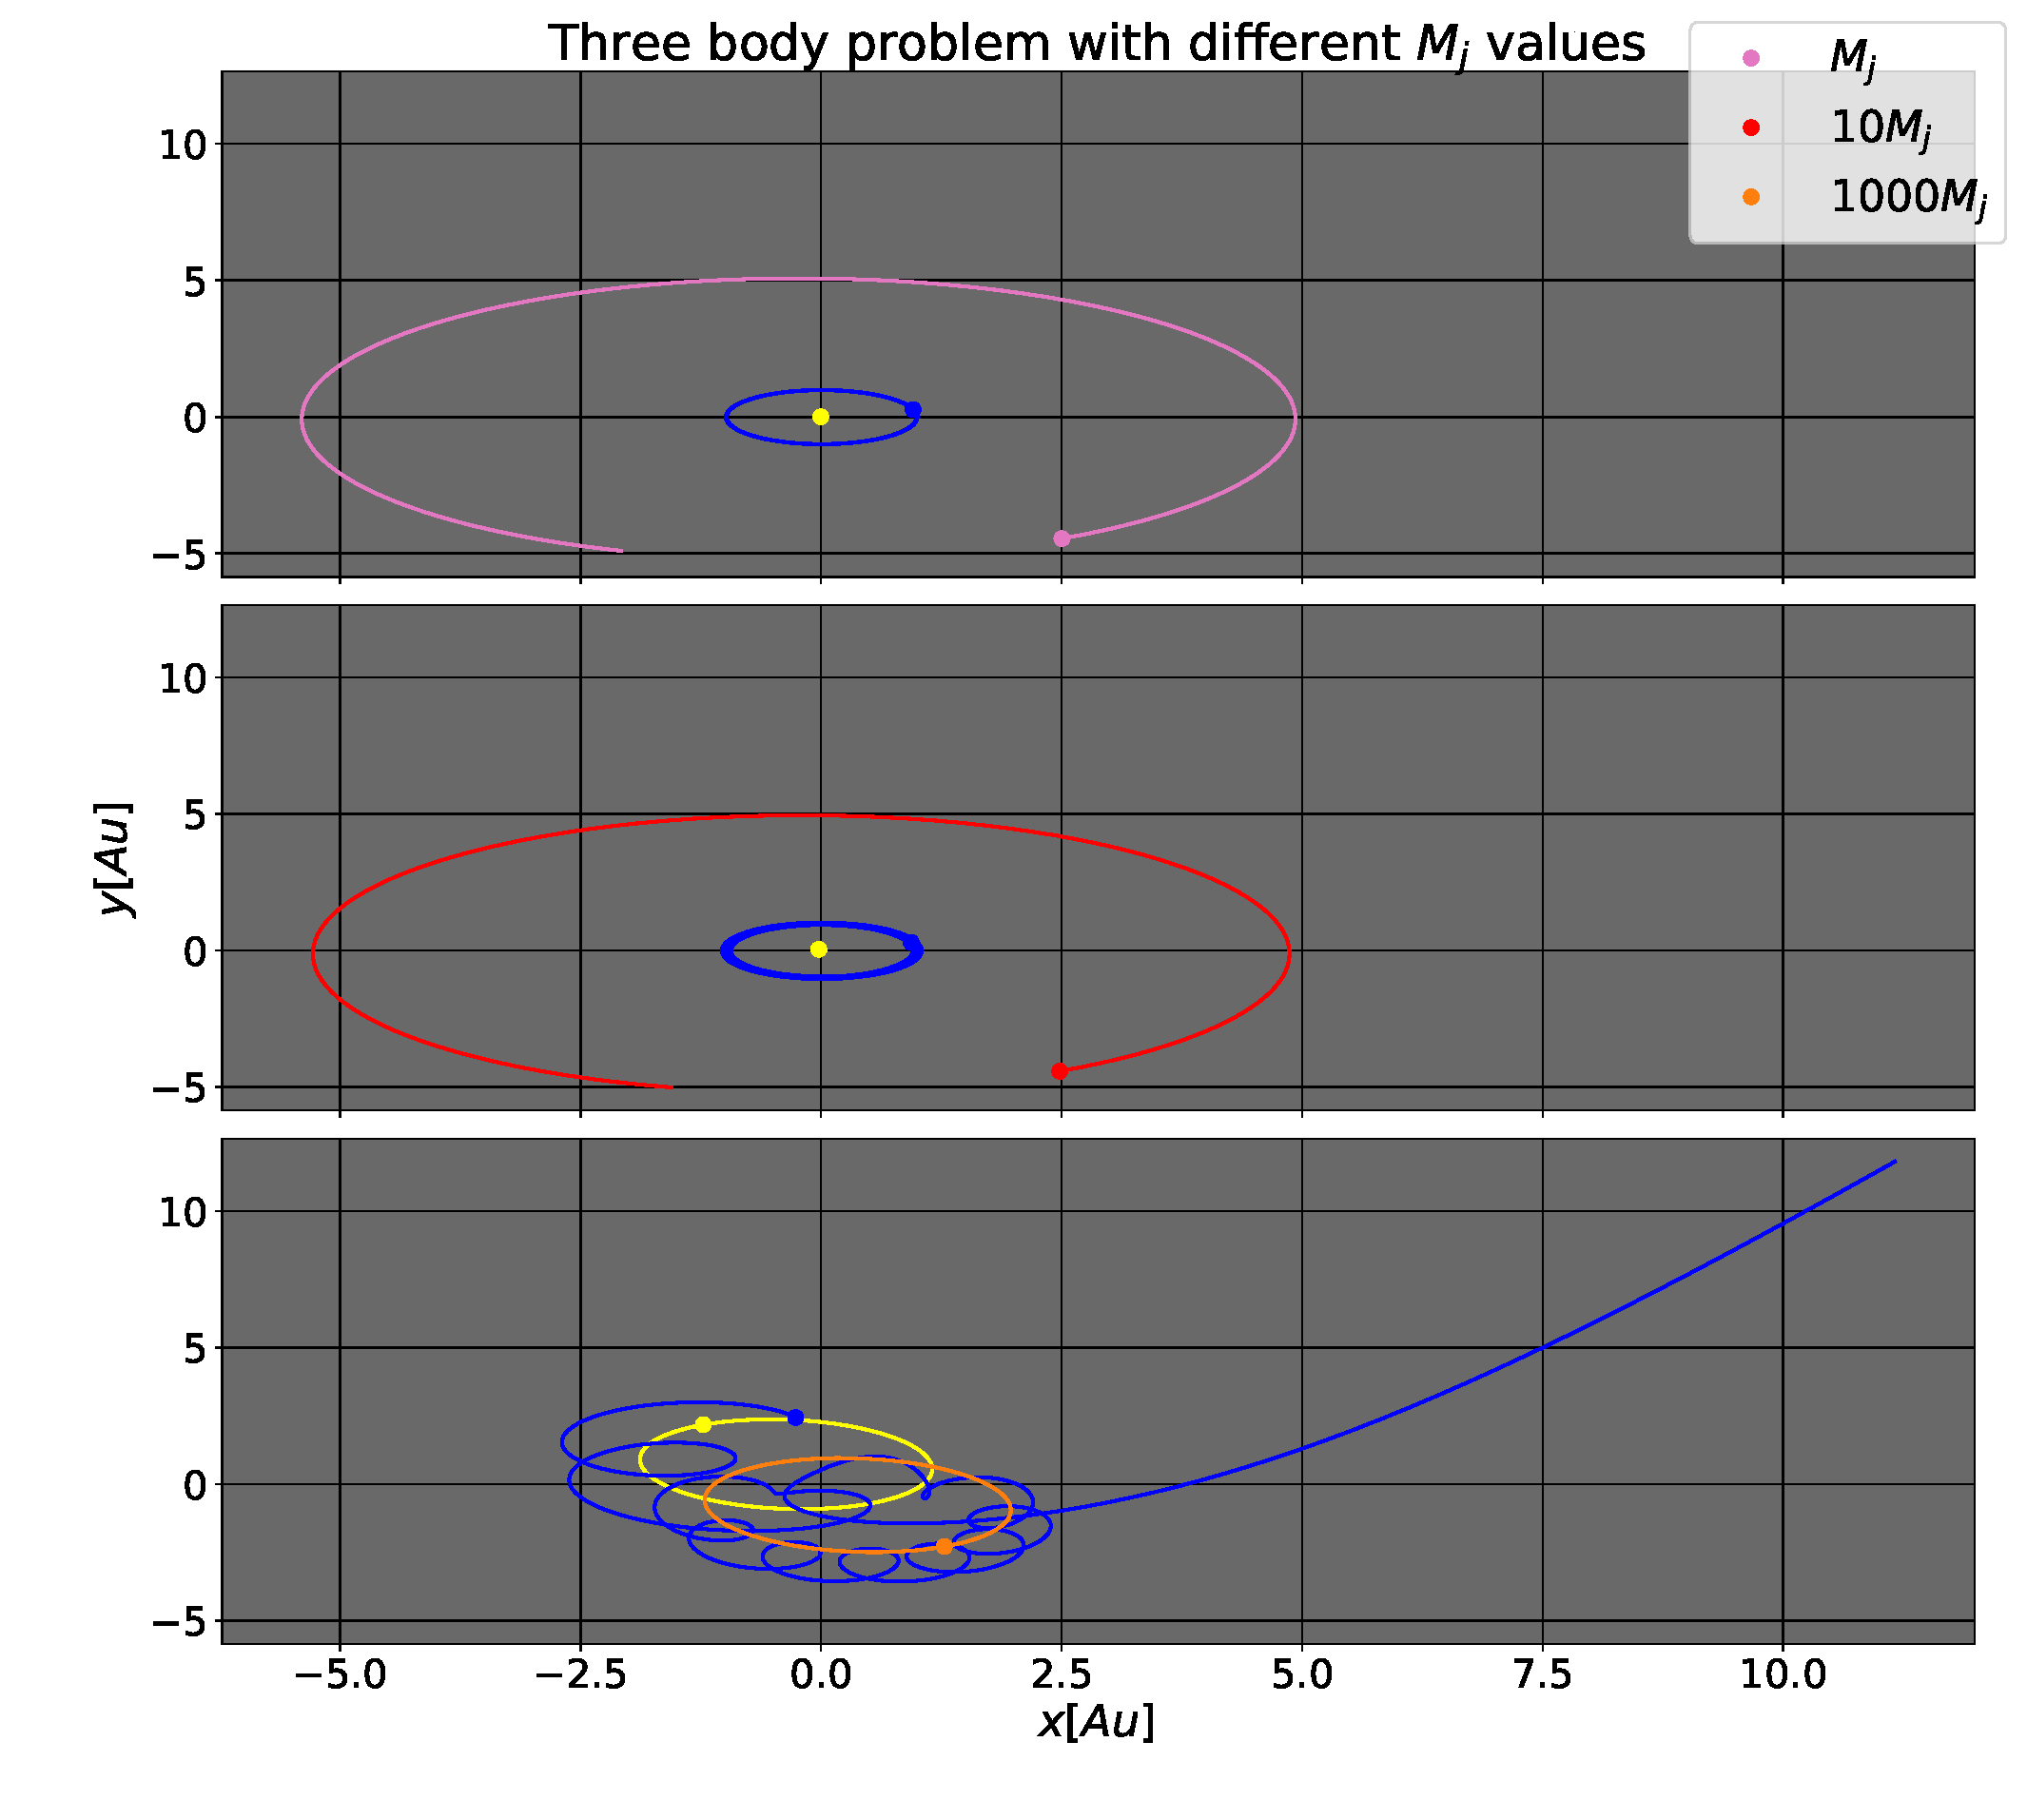
\includegraphics[width=0.9\textwidth]{../figures/three_body_problem.pdf}
    \caption{Plot of the simulated orbit of the Sun, Earth and Jupiter system for 10 years with: \textbf{top:} Jupiter's usual mass, $M_j$, \textbf{middle:} $10M_j$ \textbf{bottom:} $1000M_j$. The initial position of the Sun is not in the center in the bottom subfigure, as Jupiter is so massive in this case that the center of mass is moved to almost equidistantly between it and the Sun.}
    \label{fig:three-body-problem}
\end{figure}

\subsubsection{Extending to the entire solar system}

Extending the framework of the three-body problem, the entire solar system can be simulated. 248 years of simulation allows for one full orbit of Pluto, as shown in \cref{fig:solar-system1}. Since the innermost planets have orbits that are difficult to make out, they are shown more accurately in \cref{fig:solar-system2}.

\begin{figure}[htb!]
    \centering
    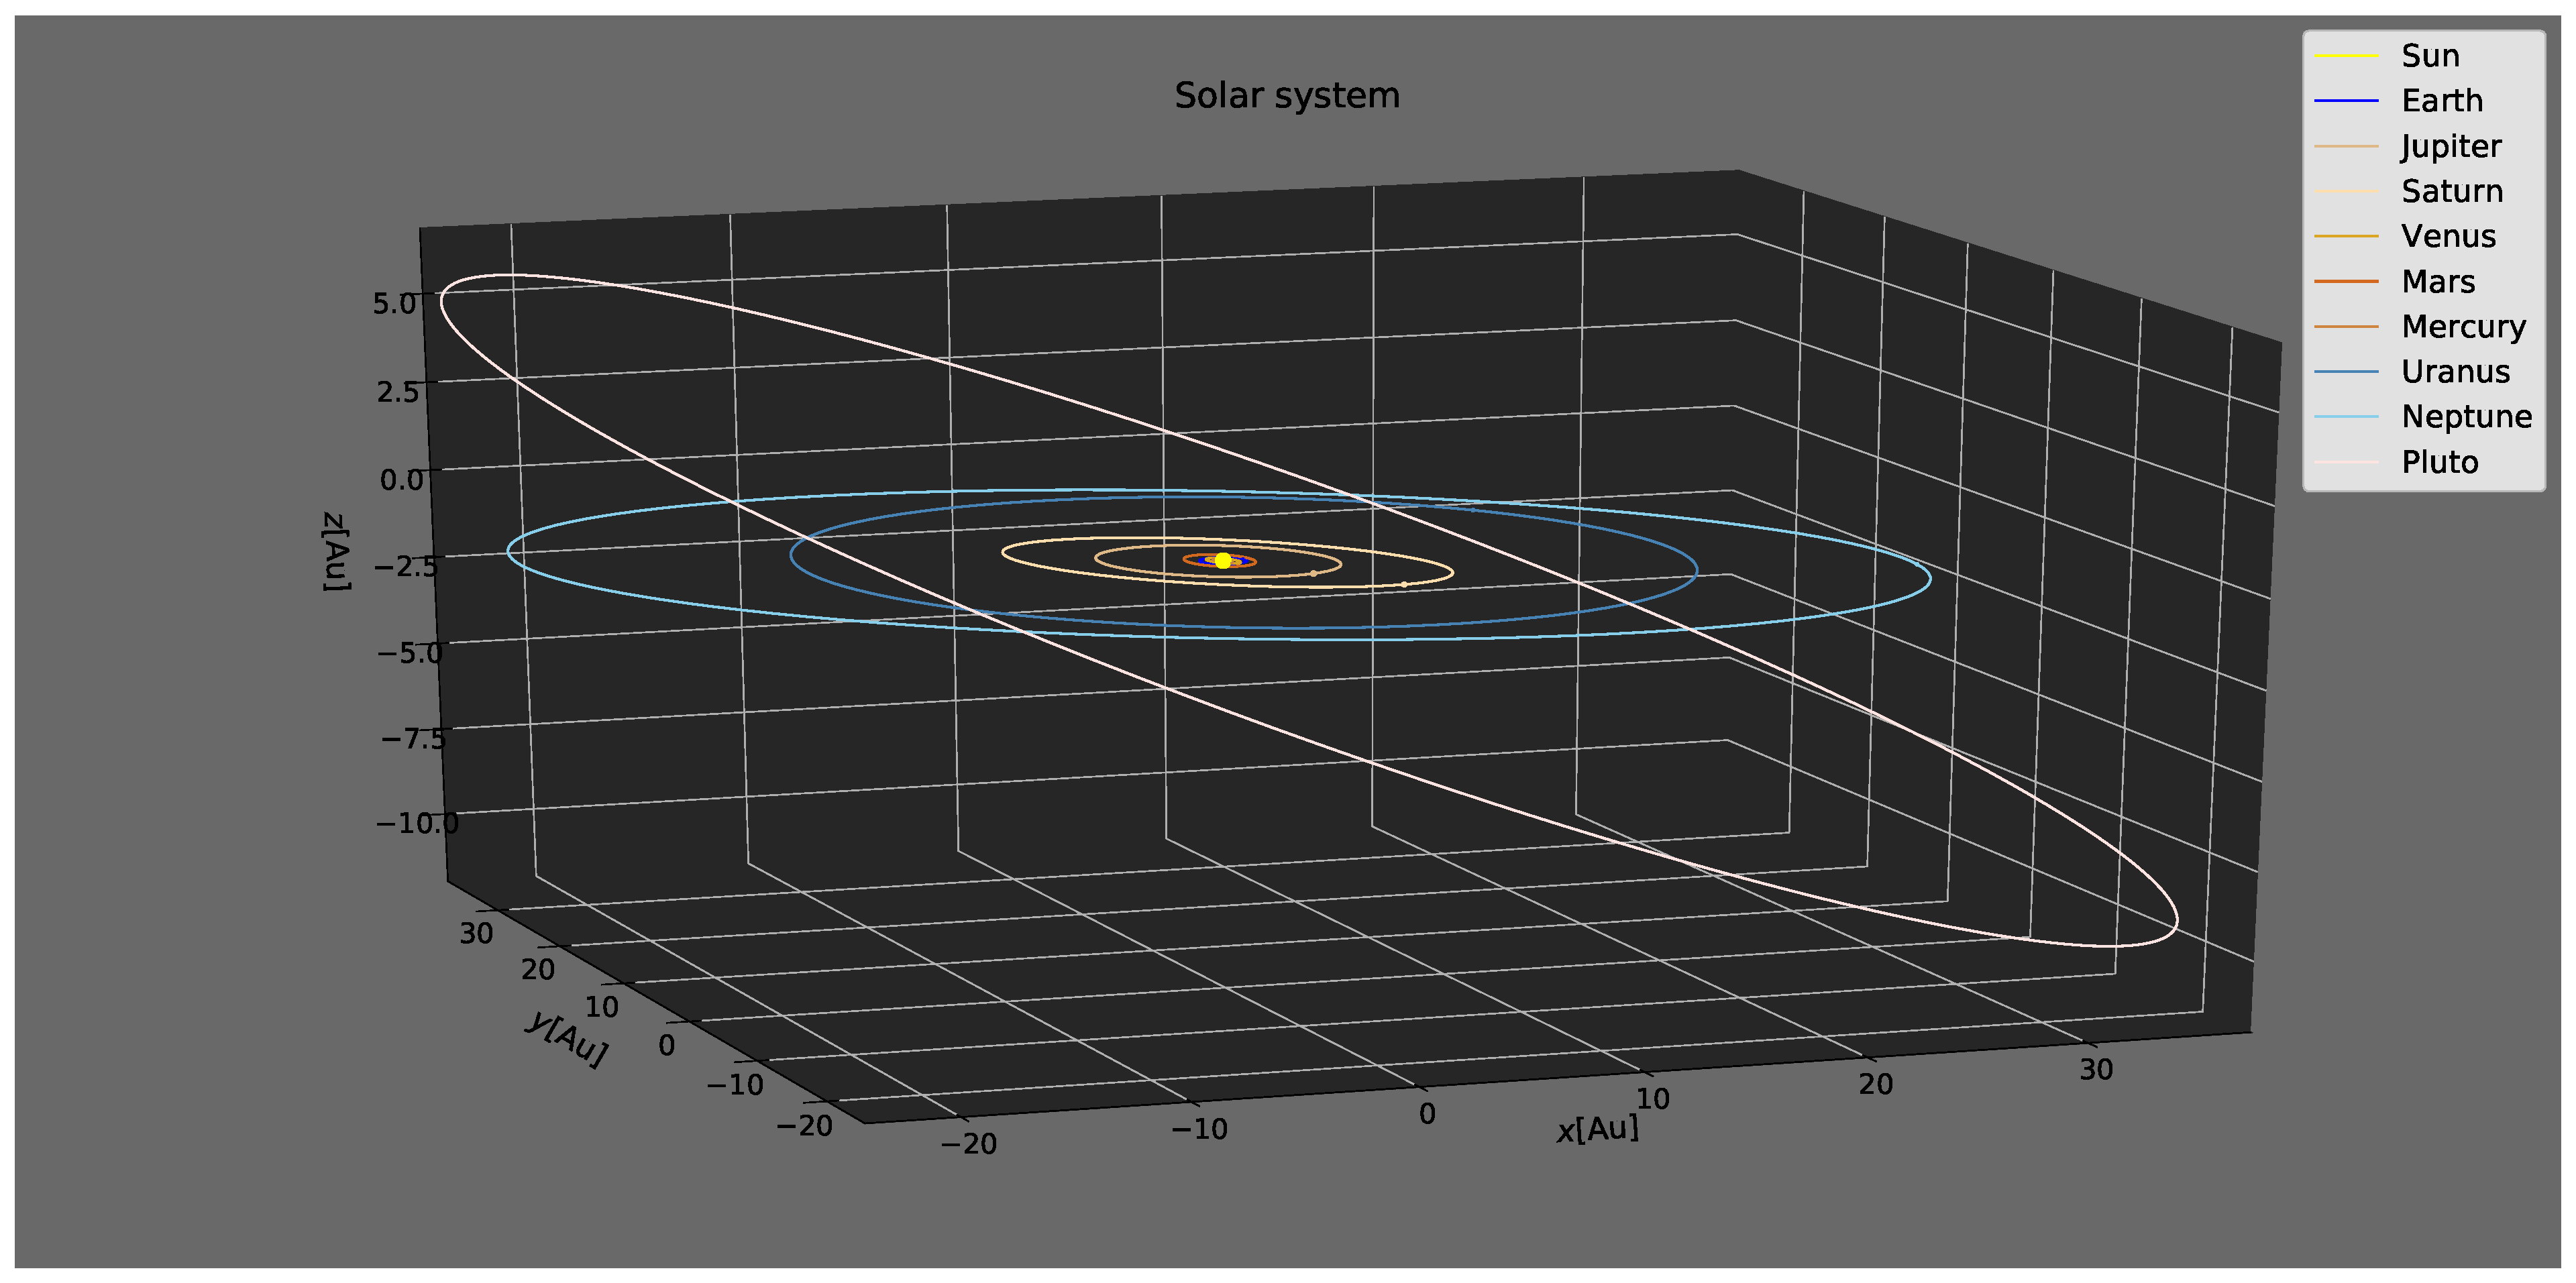
\includegraphics[trim=5.cm 0.cm 0.cm 0.cm, clip,width=0.8\textwidth]{../figures/solar_system1.pdf}
    \caption{Simulation of all the planets in the solar system. The time is 248 years.}
    \label{fig:solar-system1}
\end{figure}

\begin{figure}[htb!]
    \centering
    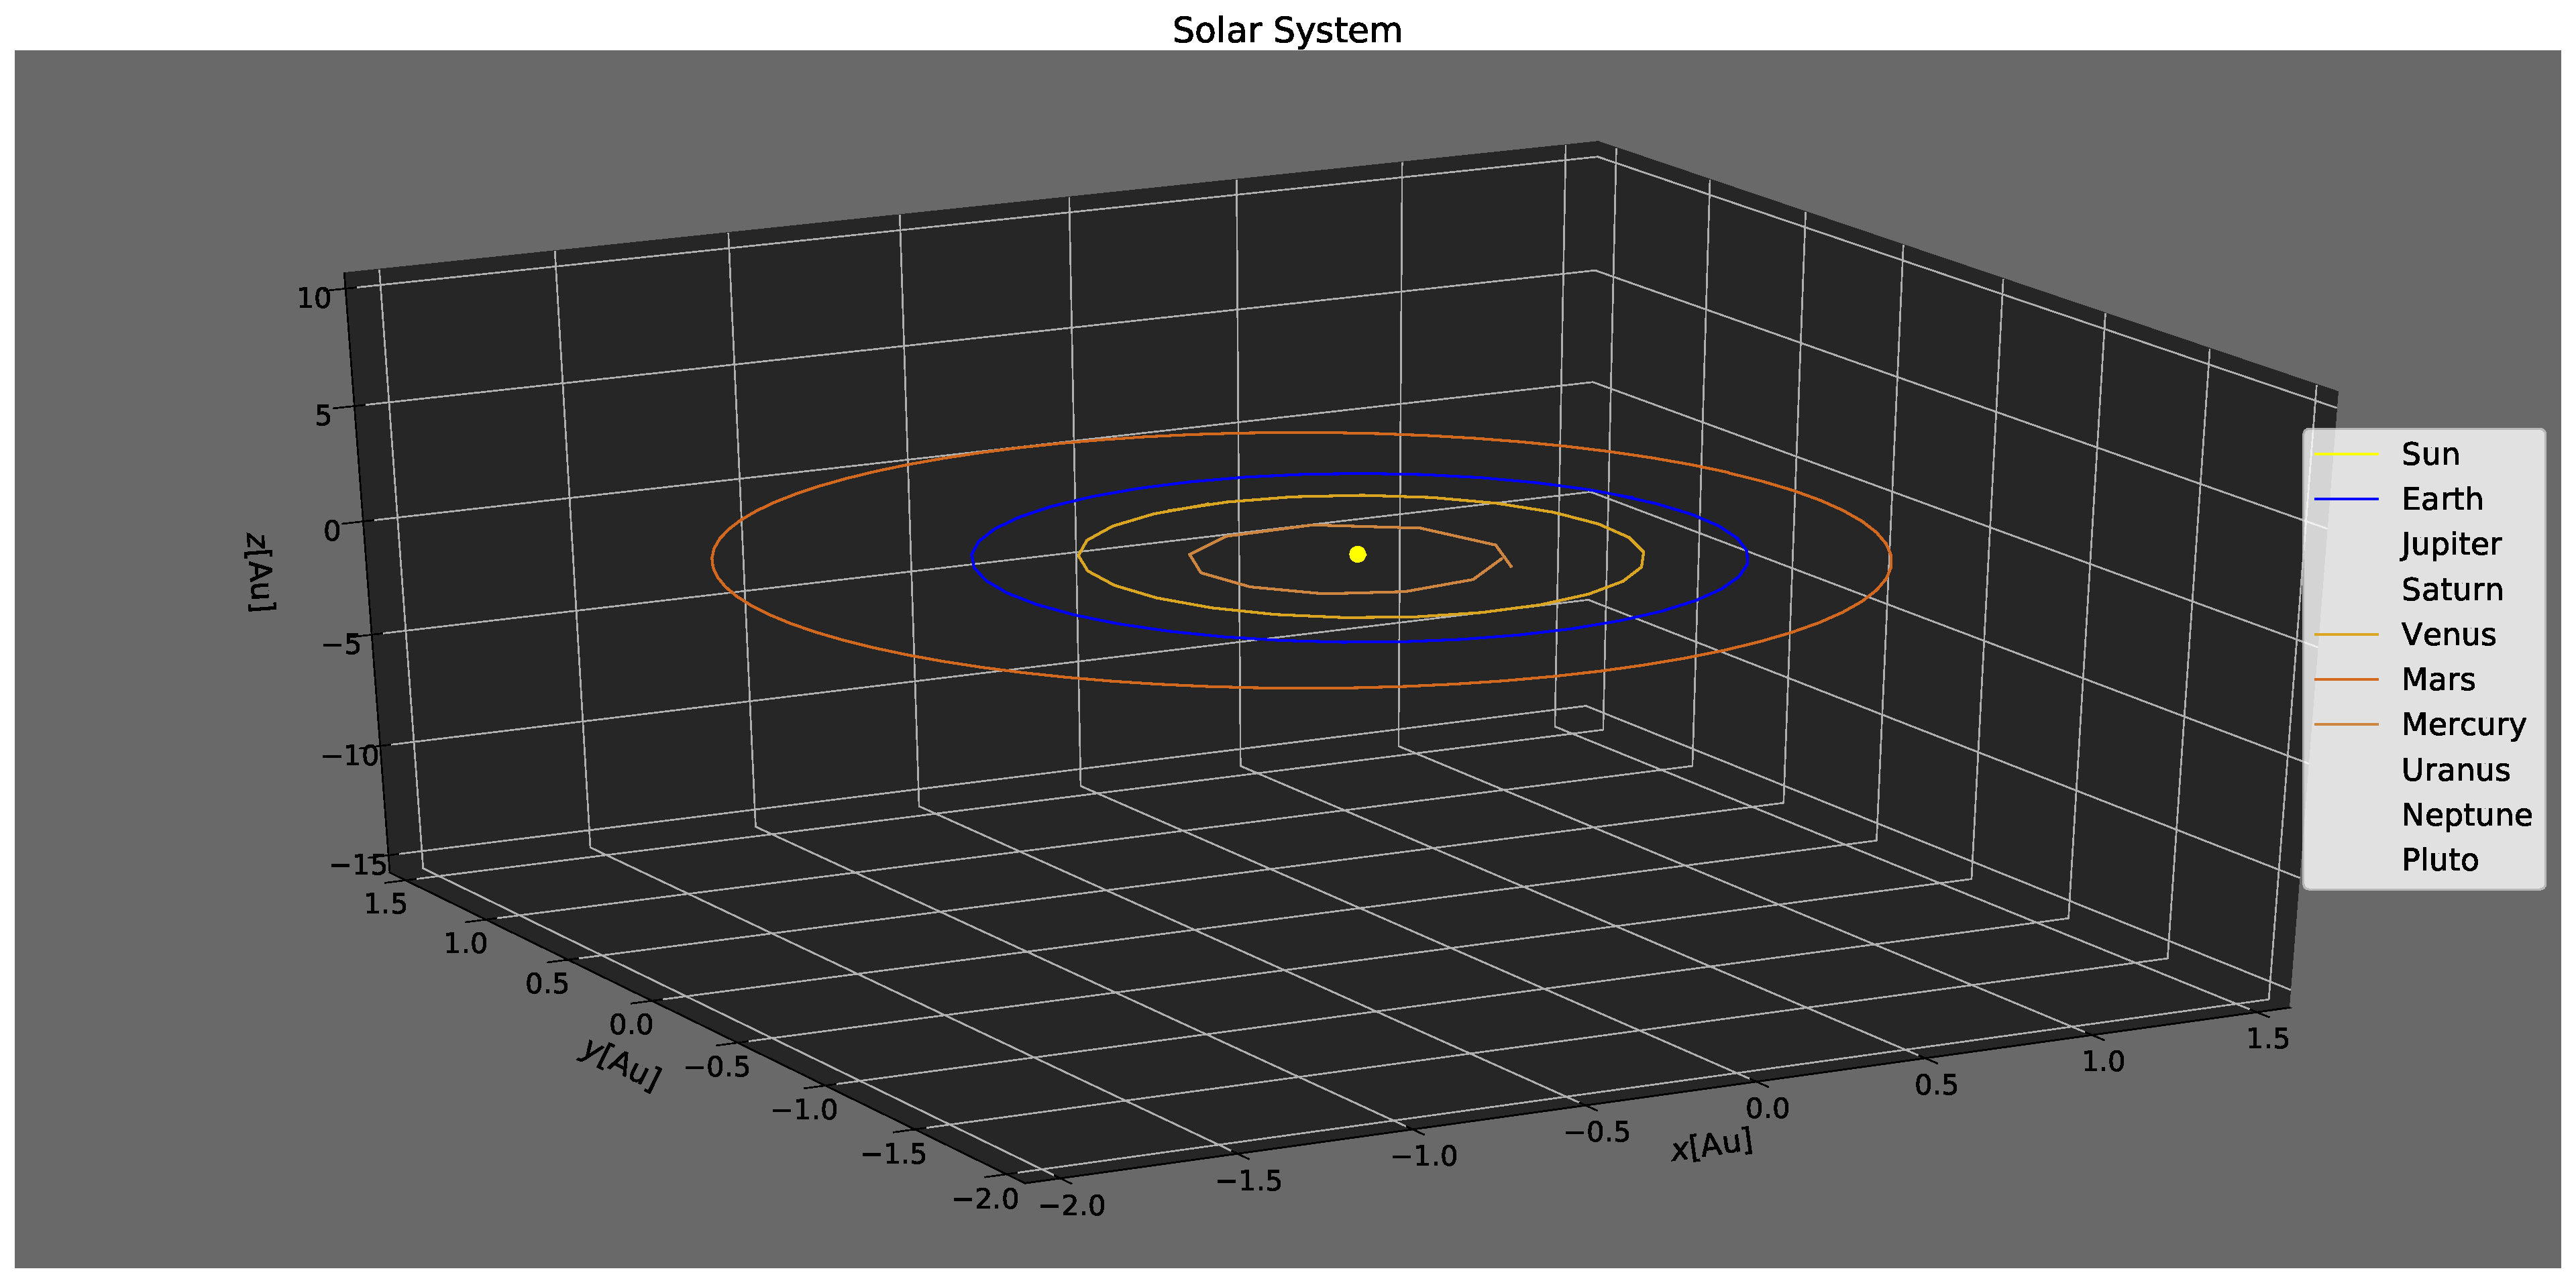
\includegraphics[trim=5.cm 0.cm 0.cm 0.cm, clip,width=0.8\textwidth]{../figures/solar_system2.pdf}
    \caption{The same plot from \cref{fig:solar-system1}, zoomed in to reveal the innermost planets.}
    \label{fig:solar-system2}
\end{figure}

\subsection{Perihelion Precession}

Applying the relativistic correction in \cref{eq:rel-correction} to the classical Newtonian equation of gravity, we simulated one century of only Mercury and the Sun. Starting at perihelion, the point closest to the Sun, we simulated with relativistic corrected gravity and without. The angles between the coordinates of the first perihelion and the coordinates of subsequent perihelions are plotted in \cref{fig:perihelion-precession}, against the observed $43''$ precession per century.


\begin{figure}[htb!]
    \centering
    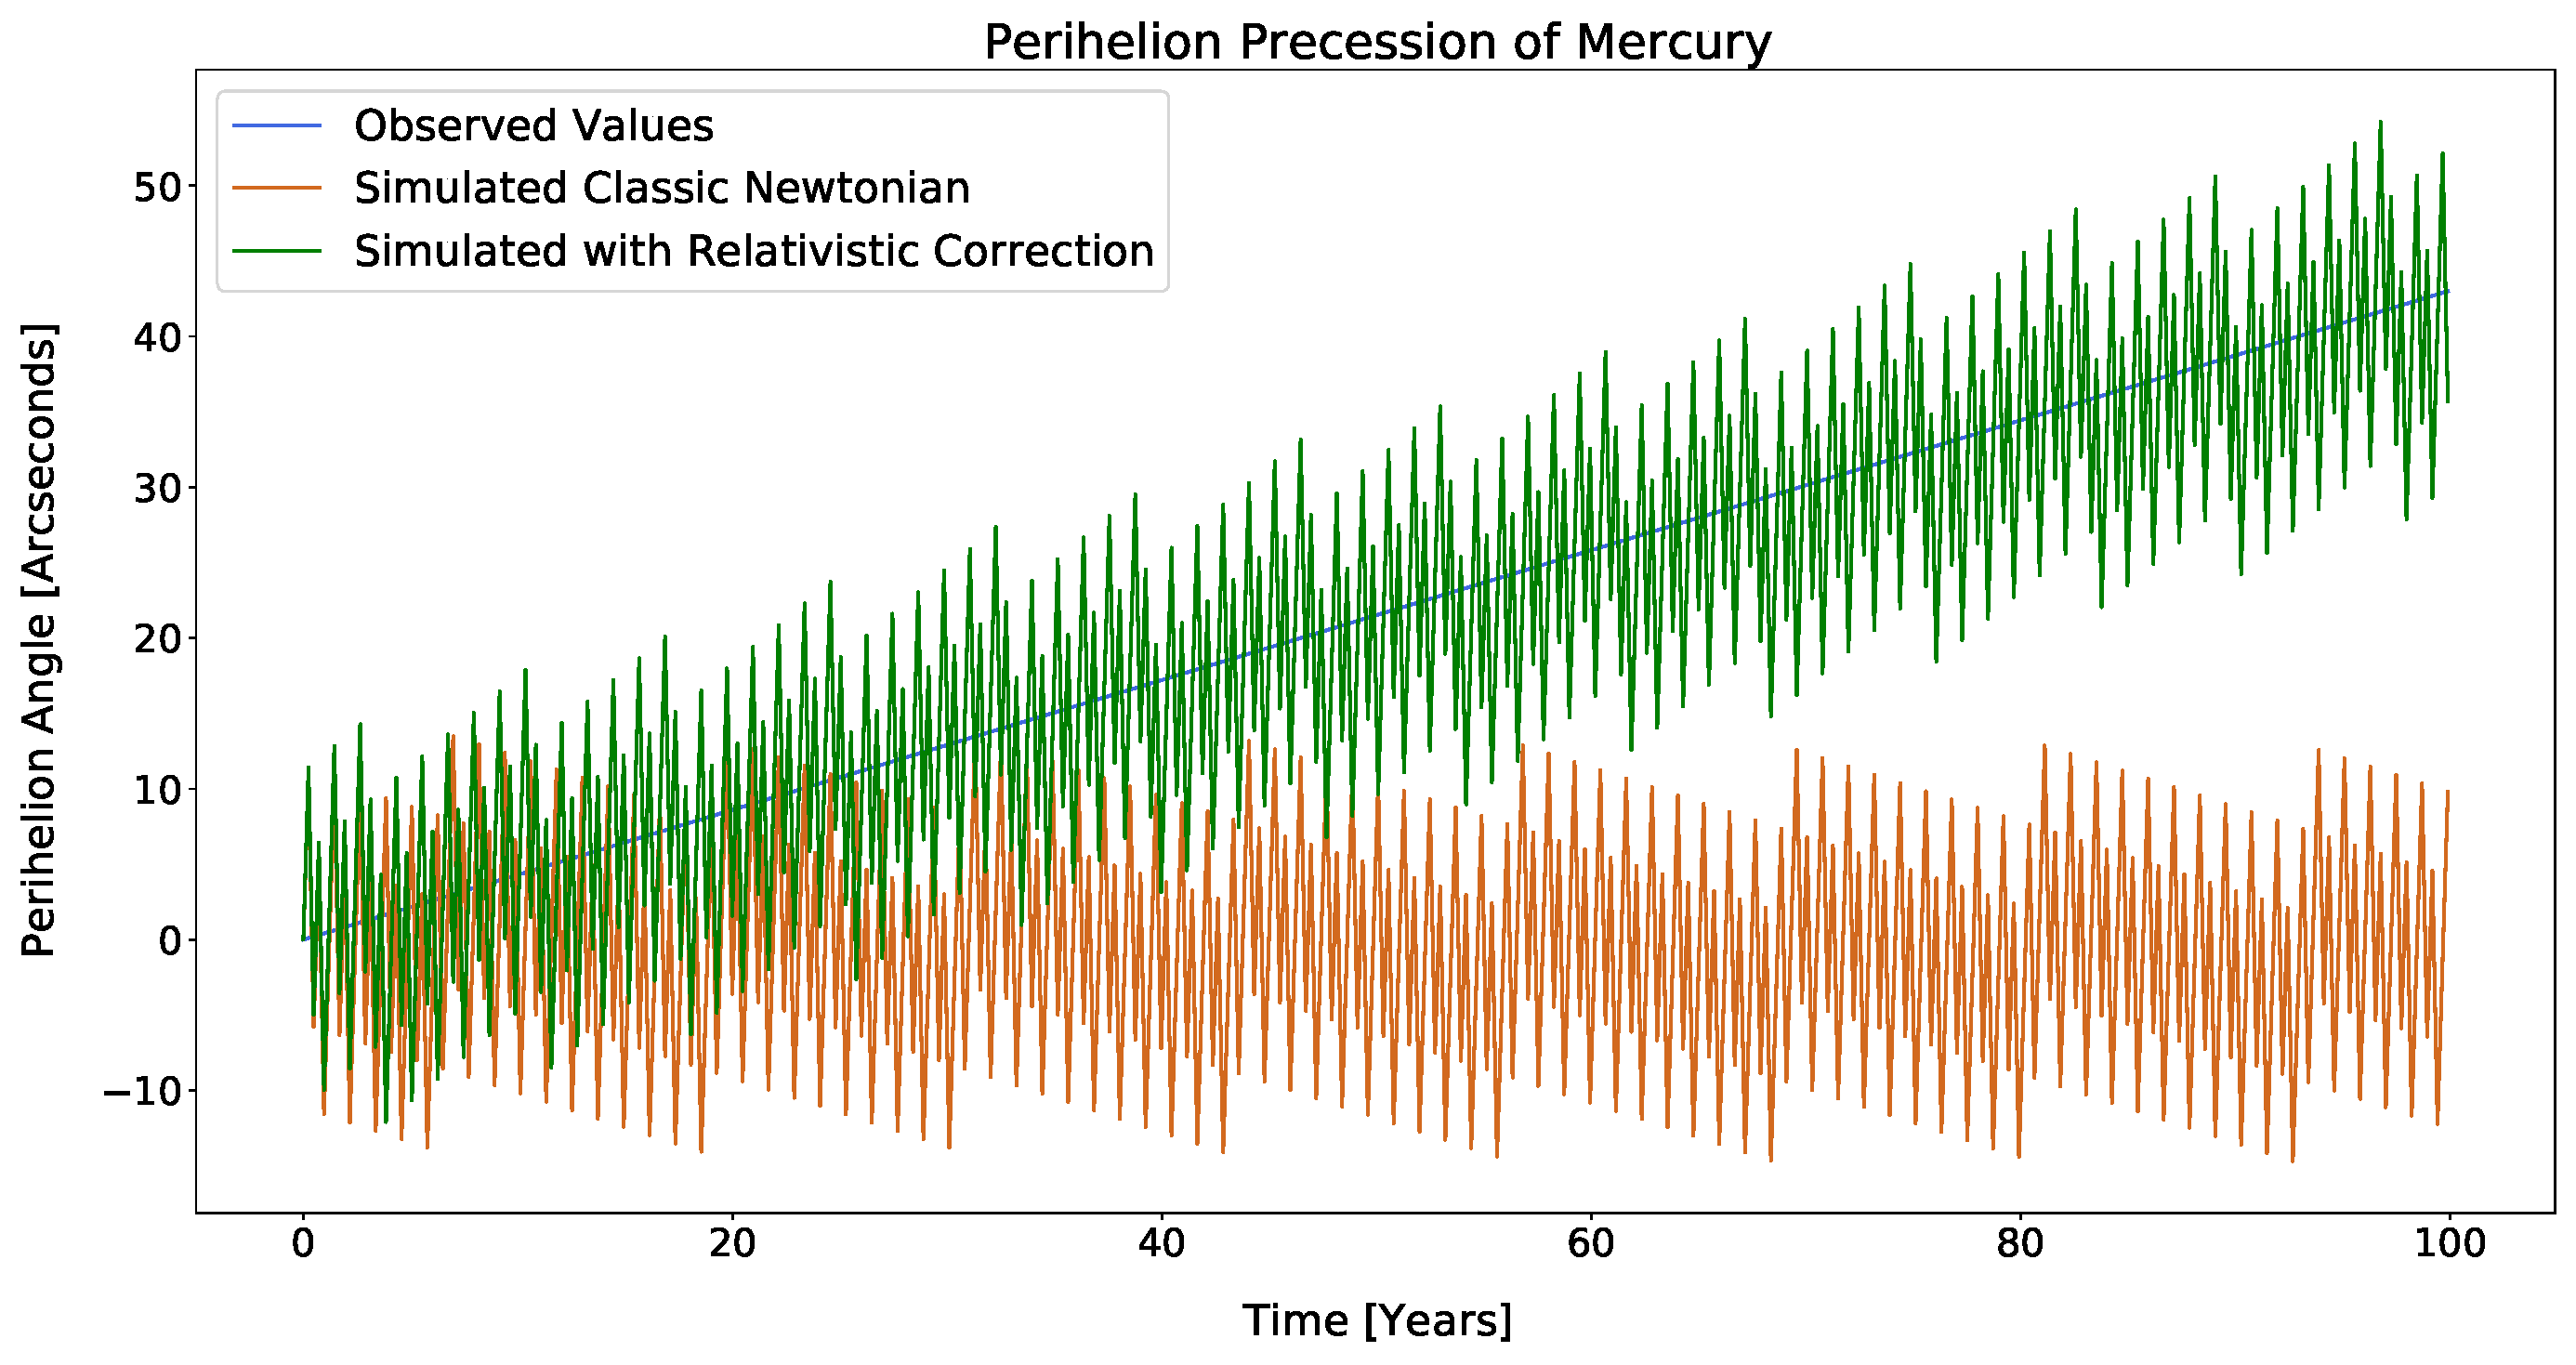
\includegraphics[width=1.0\textwidth]{../figures/3-10^7 perihelion.pdf}
    \caption{Plot of the perihelion angle of Mercury as a function of time, for observed and simulated values, with and without relativistic correction. While the simulated data is noisy, it is clear that the relativistic correction follows the observed values closely.}
    \label{fig:perihelion-precession}
\end{figure}



\end{document}
